\documentclass[aspectratio=169,9pt]{beamer}

\usepackage[utf8]{inputenc}
\usepackage{amssymb,latexsym,amsmath}
\usepackage{graphicx}
\graphicspath{ {./figures/} }
\usepackage{caption}
\usepackage{subcaption}
\captionsetup{font=tiny,labelfont=tiny}
\usepackage[style=apa,
			sorting=nyt,
			date=year,
			bibencoding=utf8,
			isbn=false,
			eprint=false,
			dashed=false,
			uniquelist=false,
			maxbibnames=10,
			minbibnames=1,
			maxcitenames=2,
			uniquename=init,
			giveninits=true,
			useprefix=false,
			minsortnames=1,
			maxsortnames=2]{biblatex}
\renewcommand*{\bibfont}{\footnotesize}
\renewcommand*{\citesetup}{\tiny}
\renewcommand{\cite}{\parencite}
\bibliography{References}

% Beamer theme
\usetheme[titleformat=smallcaps,
			sectionpage=progressbar,
			subsectionpage=progressbar,
			progressbar=frametitle,
			numbering=fraction]{metropolis}
% FiraFonts if using pdflatex
% \usepackage{FiraSans}
% \usepackage{FiraMono}

% Information to be included in the title page:
\title[Thesis Defence]{A theoretical study of the implications of resource competition for adaptive therapy of castration-resistant prostate cancer}
\subtitle{Thesis Defence}
\author[Harshavardhan BV]{Harshavardhan BV\\
Supervisor: Prof. Sutirth Dey}
\date{July 2021}
\institute{IISER Pune}

\begin{document}

\frame{\titlepage}

\section{Introduction}

\begin{frame}{Conventional and adaptive Therapy}
  \begin{columns}
    \begin{column}{0.45\textwidth}
      \begin{itemize}
        \item Conventional therapy @ MTD $\rightarrow$\\
        $\downarrow$ tumour burden \cite{Frei}
        \item Heterogenous sensitivity $\rightarrow$\\
        sens. $\times$ $\rightarrow$ resst. \cite{Scott}
        \item AT = $\downarrow$ , $\sim$ dose $\rightarrow$ sens. $\checkmark$ \cite{Gatenby}
        \item Drug holiday - sens. $\rightarrow\ \downarrow$ resst.
        \item AT outcome $\leftarrow$ competition
      \end{itemize}
    \end{column}
    \begin{column}{0.55\textwidth}
      \begin{figure}[h]
        \centering
        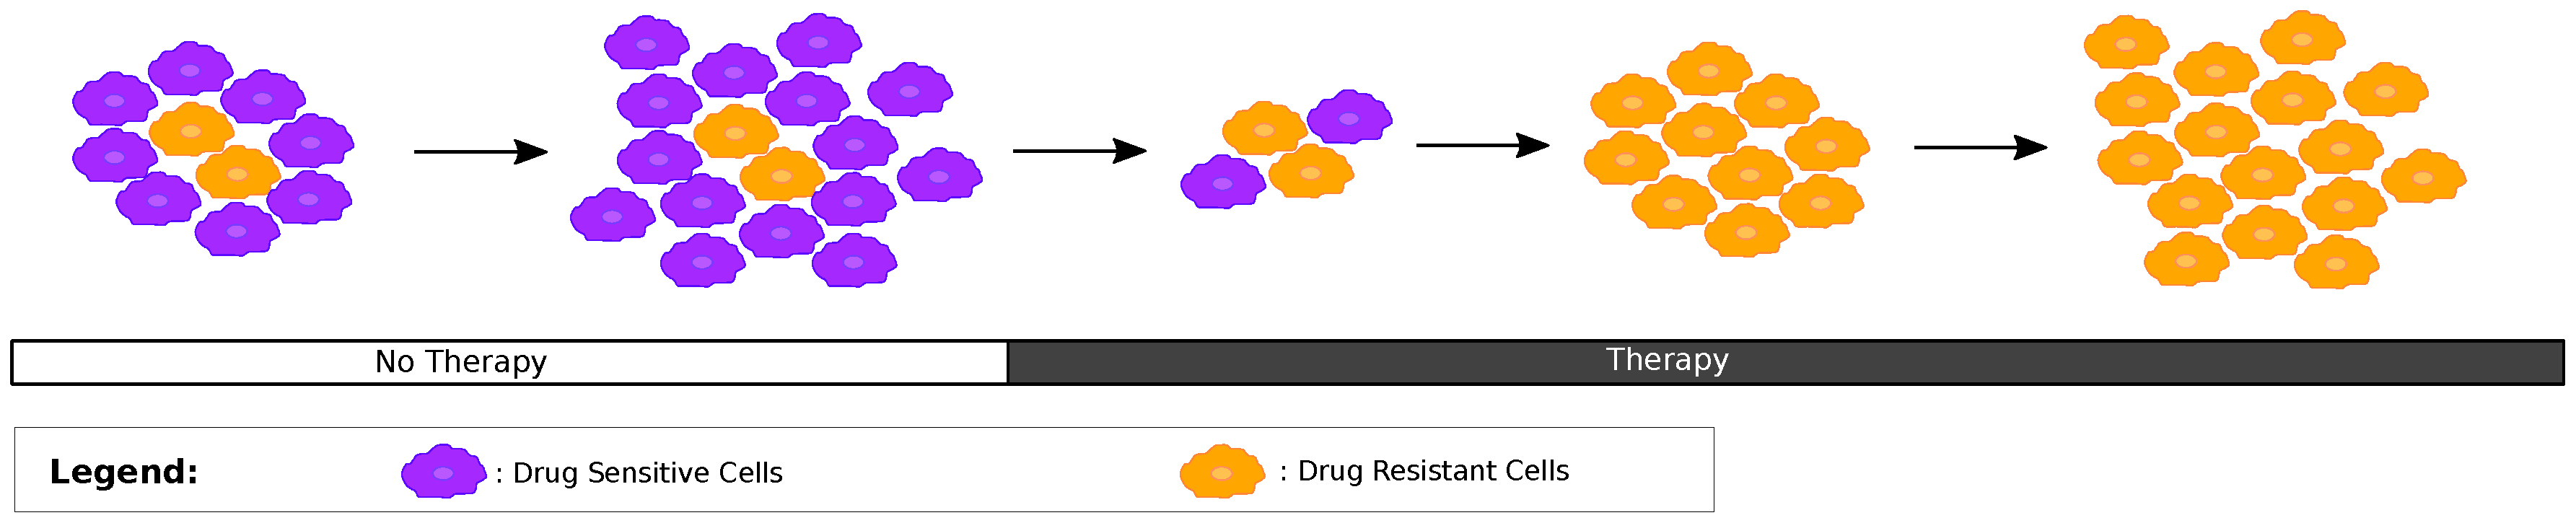
\includegraphics[width=\textwidth]{compe_release}
        \caption{Competitive release under SOC}
      \end{figure}
      \begin{figure}[h]
        \centering
        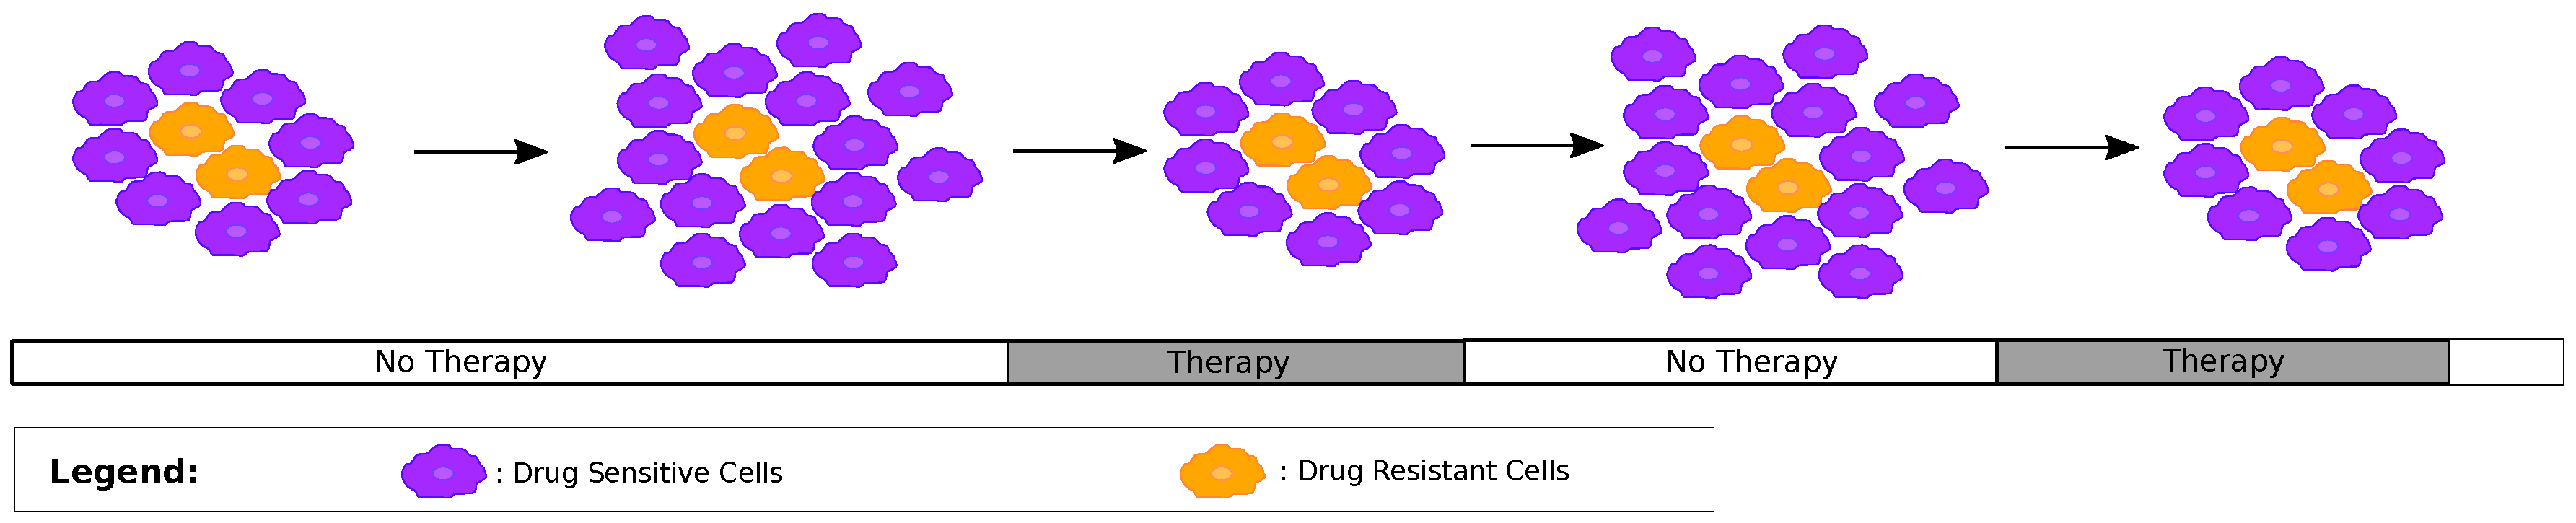
\includegraphics[width=\textwidth]{at}
        \caption{Control under AT}
      \end{figure}
    \end{column}
  \end{columns}
\end{frame}

\begin{frame}{System of study}
  \begin{itemize}
    \item Castration-Resistant Prostate Cancer (CRPC)
    \item AR pathway: prostate cells $\rightarrow$ cancer \cite{Heinlein}
    \item Therapy: ADT + Abiraterone
  \end{itemize}
  \begin{table}
    \centering
    \begin{tabular}{|l|c|c|c|c|}
    \hline
    Cell type & Test. dependent & Test. Producing & Ab. sensitive & Mechanism \\
    \hline
    $T^+$ & Yes & No & Yes & N/A \\
    $T^p$ & Yes & Yes & Yes & Cholesterol $\xrightarrow{CYP17\alpha}$ Test.\\
    $T^-$ & No & No & No & AR $\mu^n$\\
    \hline
    \end{tabular}
  \end{table}
\end{frame}

\begin{frame}{System of equations}
  \begin{columns}
    \begin{column}{0.45\textwidth}
      \begin{itemize}
        \item Logistic framework w/ dynamic carrying capacity $\approx$ env. condn.
        \item Environment = resource = $\{O_2,test\}$
        \item No $\mu^n$, no spatial structure, well mixed
        \item Defined $\mathbb{R}_{\geq 0}$, $y_i < 1 =$ extinction
      \end{itemize}
      \begin{figure}[h]
        \centering
        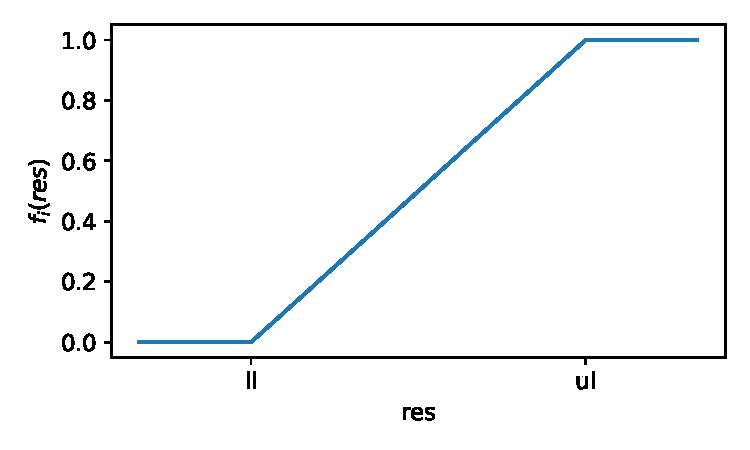
\includegraphics[width=\textwidth]{f_res}
        \caption{$f_i(res)$}
      \end{figure}
    \end{column}
    \begin{column}{0.55\textwidth}
      \begin{equation}
        \frac{dy_i}{dt} = r_i y_i (1 - \frac{\sum_j y_j}{1 + K_{i,max} f_i(O_2) f_i(test)} )- \delta_i y_i
        \label{celleq}
      \end{equation}
      \begin{equation}
        \frac{dO_2}{dt} = p_{O_2} - \sum_i \mu_{O_2,i} y_i - \lambda_{O_2} O_2
        \label{o2eq}
      \end{equation}
      \begin{equation}
        \frac{dtest}{dt} = p_{test} y_{T^p} - \sum_i \mu_{test,i} y_i - \lambda_{test} test
        \label{testeq}
      \end{equation}
      \begin{equation}
        f_i(res) = \begin{cases}
          1 &\text{if } ul_{res,i} \leq res\\
          \frac{res-ll_{res,i}}{ul_{res,i}-ll_{res,i}} &\text{if } ll_{res,i} < res < ul_{res,i}\\
          0 &\text{if } res \leq ll_{res,i}\\
        \end{cases}
        \label{freseq}
      \end{equation}
      $i \in \{T^+,T^p,T^-\}$ and $res \in \{O_2,test\}$.
    \end{column}
  \end{columns}
\end{frame}


\section{Cell-types Interactions and Competition outcomes}

\begin{frame}{$T^p$ - $T^-$ Cases}
  \begin{figure}[h]
    \centering
    \begin{subfigure}[b]{0.48\textwidth}
      \centering
      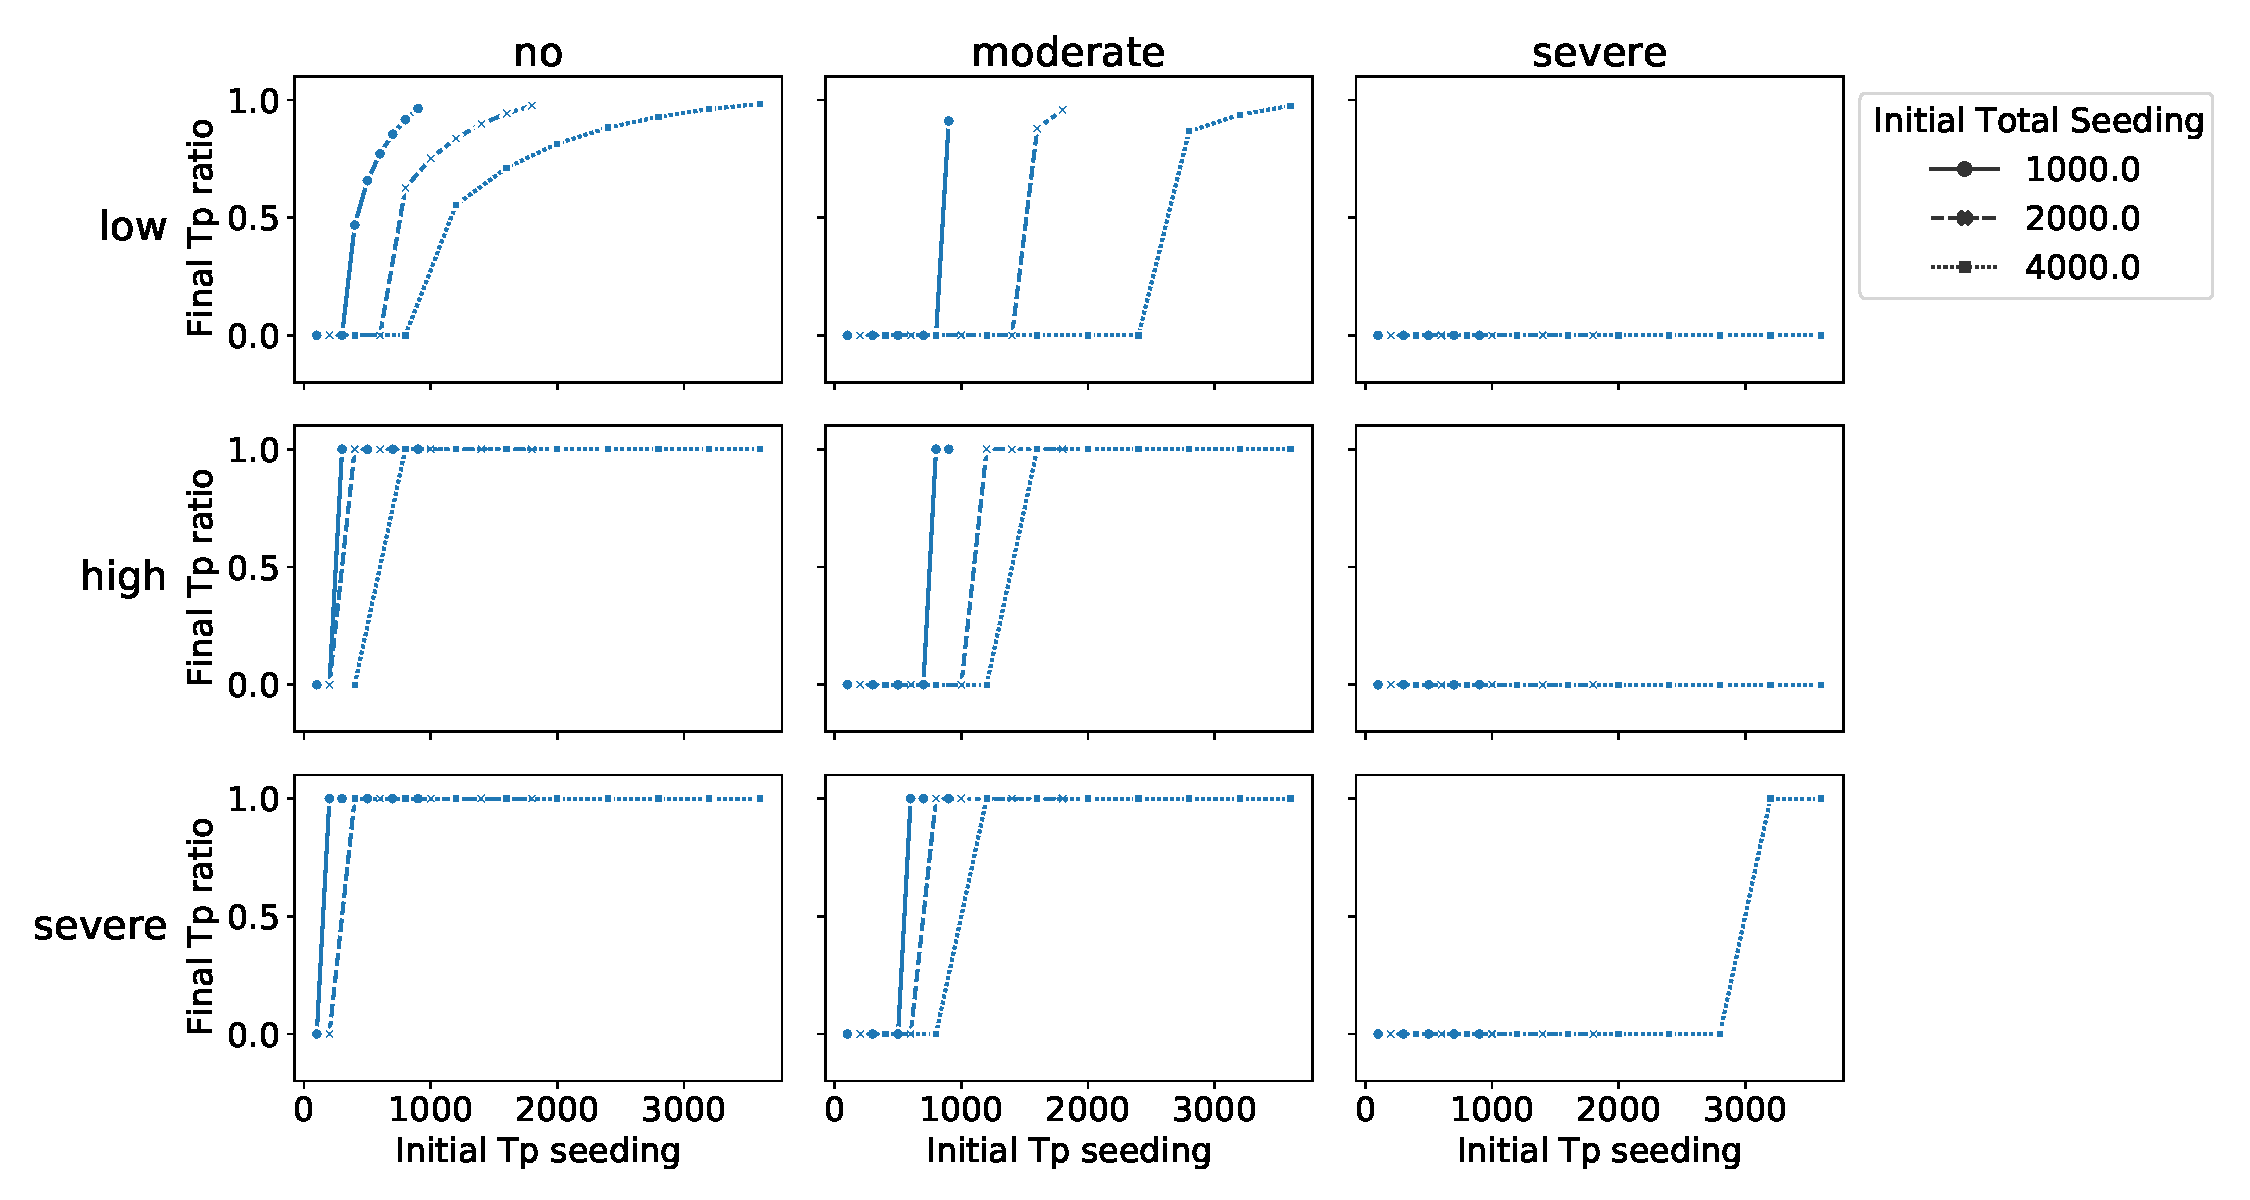
\includegraphics[width=\textwidth]{Tpro-Tneg_cases_normal}
      \caption{normal prodn.}
    \end{subfigure}
    \begin{subfigure}[b]{0.48\textwidth}
      \centering
      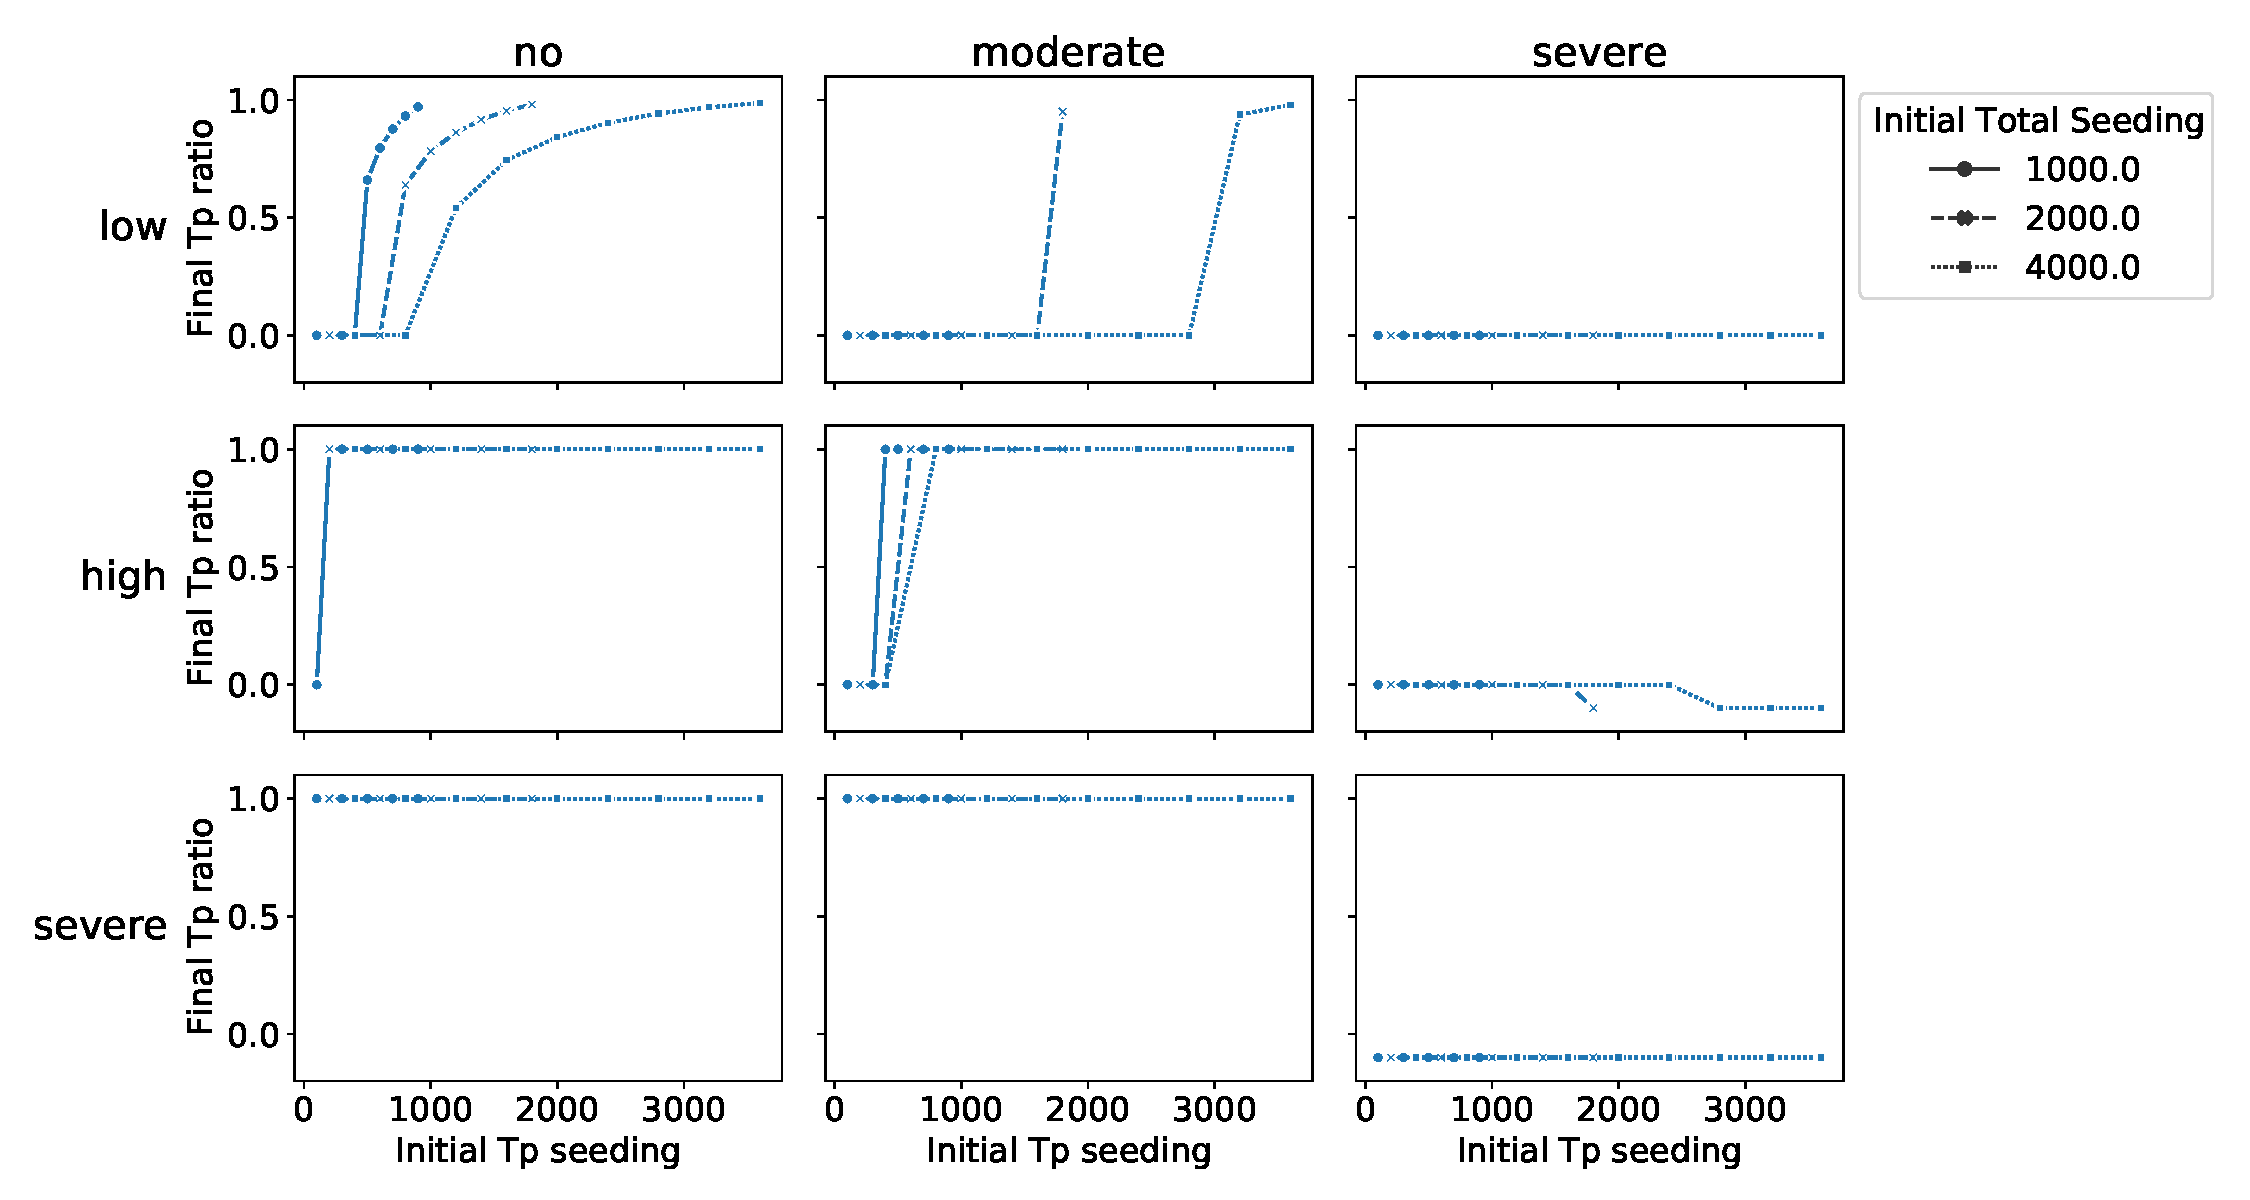
\includegraphics[width=\textwidth]{Tpro-Tneg_cases_poor}
      \caption{poor prodn.}
    \end{subfigure}
    \caption{Final $T^p$ ratio of pairwise $T^p - T^-$. SF: $O_2$ prodn., C: $T^p\ test$ limits, R: $T^-\ O_2$ limits.}
  \end{figure}
  \begin{columns}
    \begin{column}{0.5\textwidth}
      \begin{itemize}
        \item Coexist: $T^p$ no/mod. + $T^-$ low
      \end{itemize}
    \end{column}
    \begin{column}{0.5\textwidth}
      \begin{itemize}
        \item Tot. popn. vs Initial propn.
      \end{itemize}
    \end{column}
  \end{columns}
\end{frame}


\begin{frame}[allowframebreaks]{$T^+$ - $T^p$ Cases}
  \begin{figure}[h]
    \centering
    \begin{subfigure}[b]{0.48\textwidth}
      \centering
      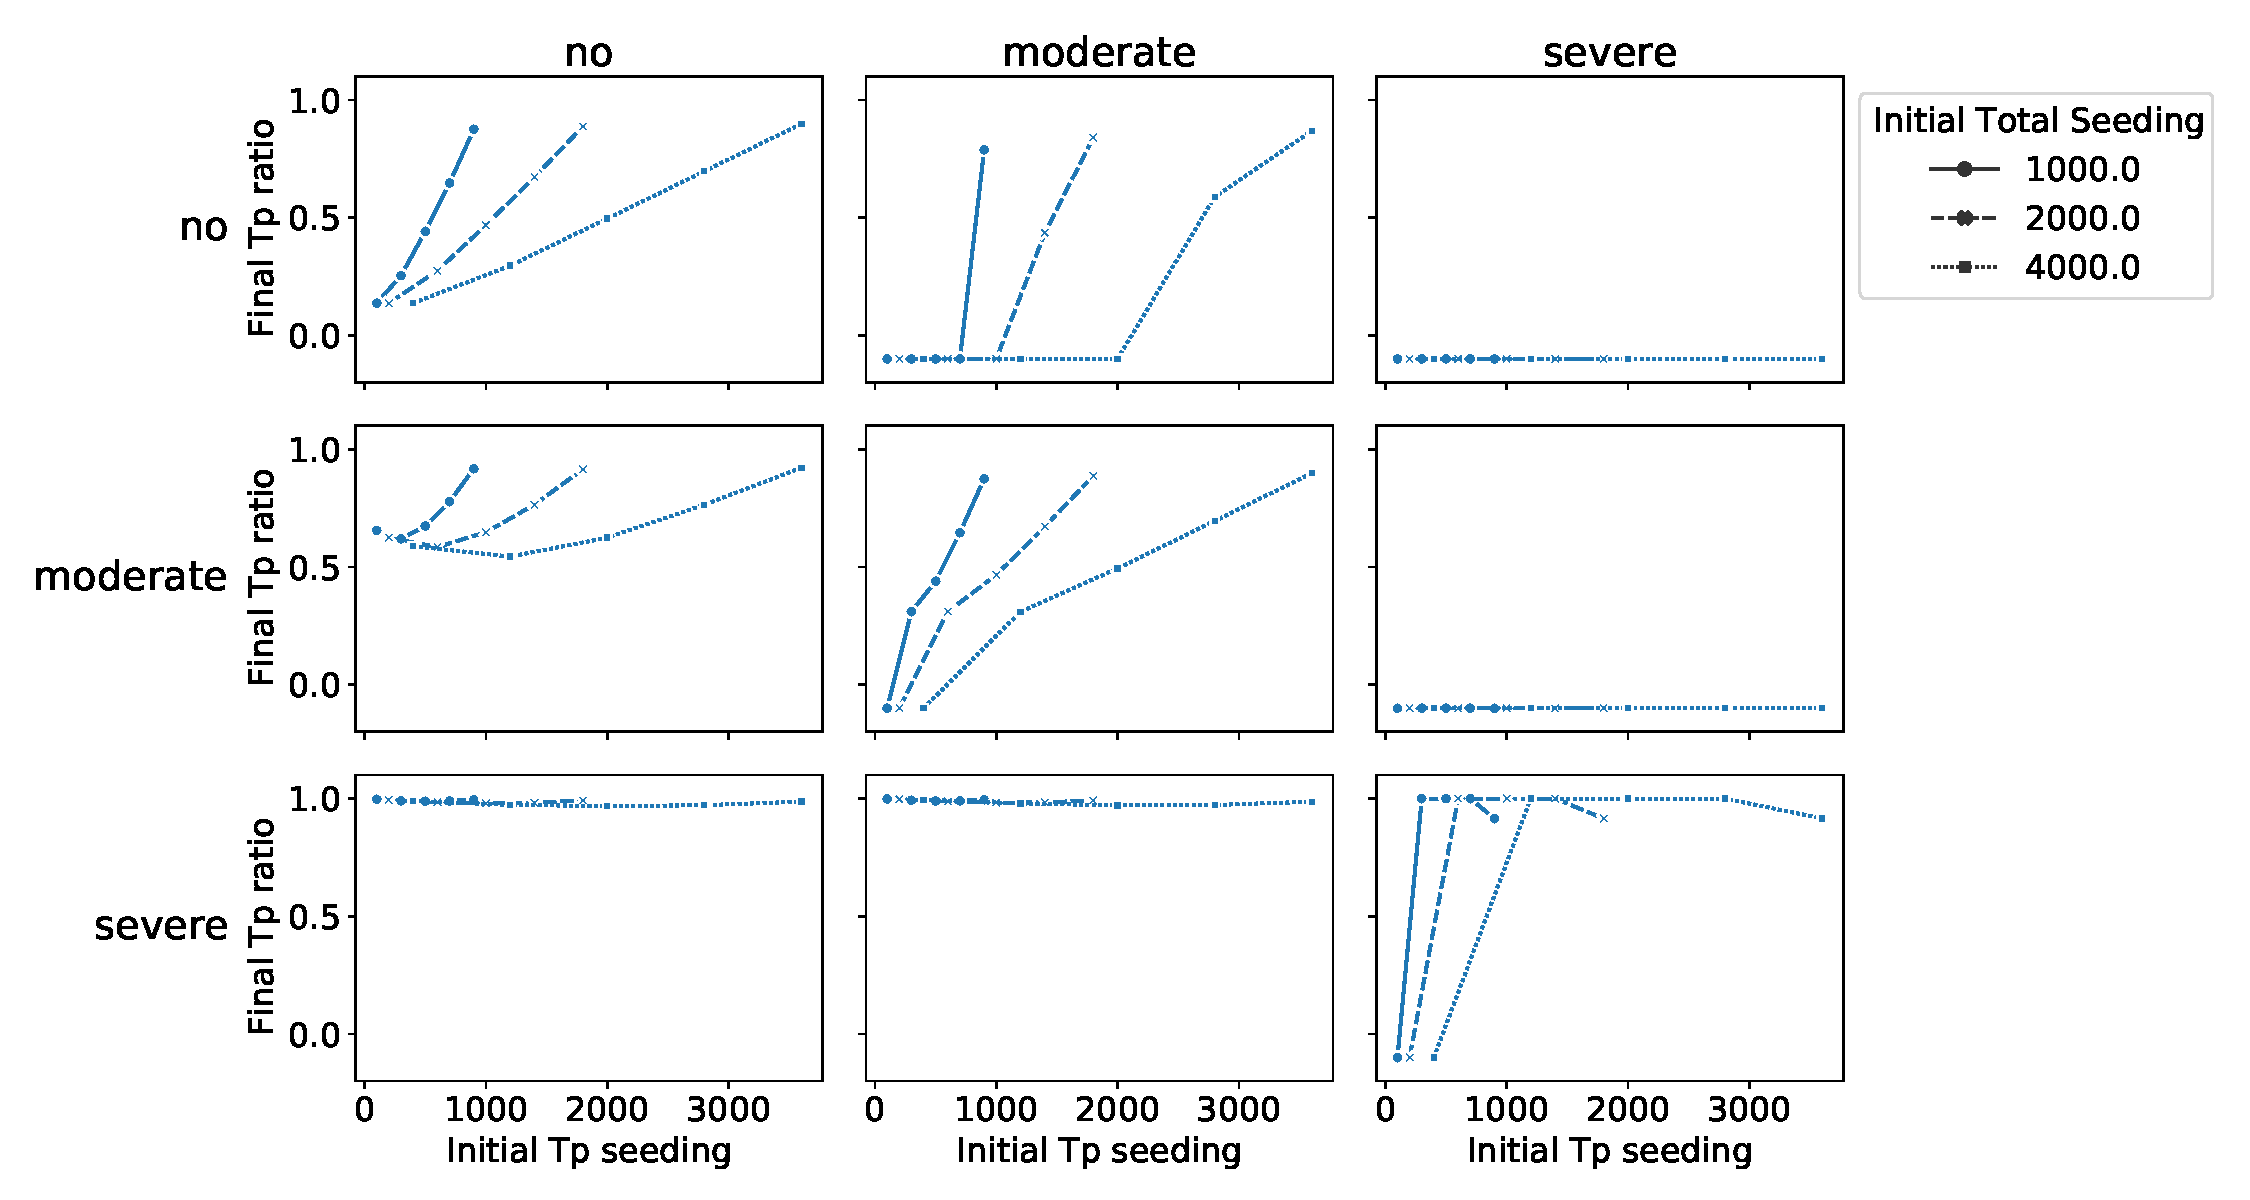
\includegraphics[width=\textwidth]{Tpos-Tpro_cases_test}
      \caption{$test$ limits. C: $T^p\ test$ limits, R: $T^+\ test$ limits}
    \end{subfigure}
    \begin{subfigure}[b]{0.48\textwidth}
      \centering
      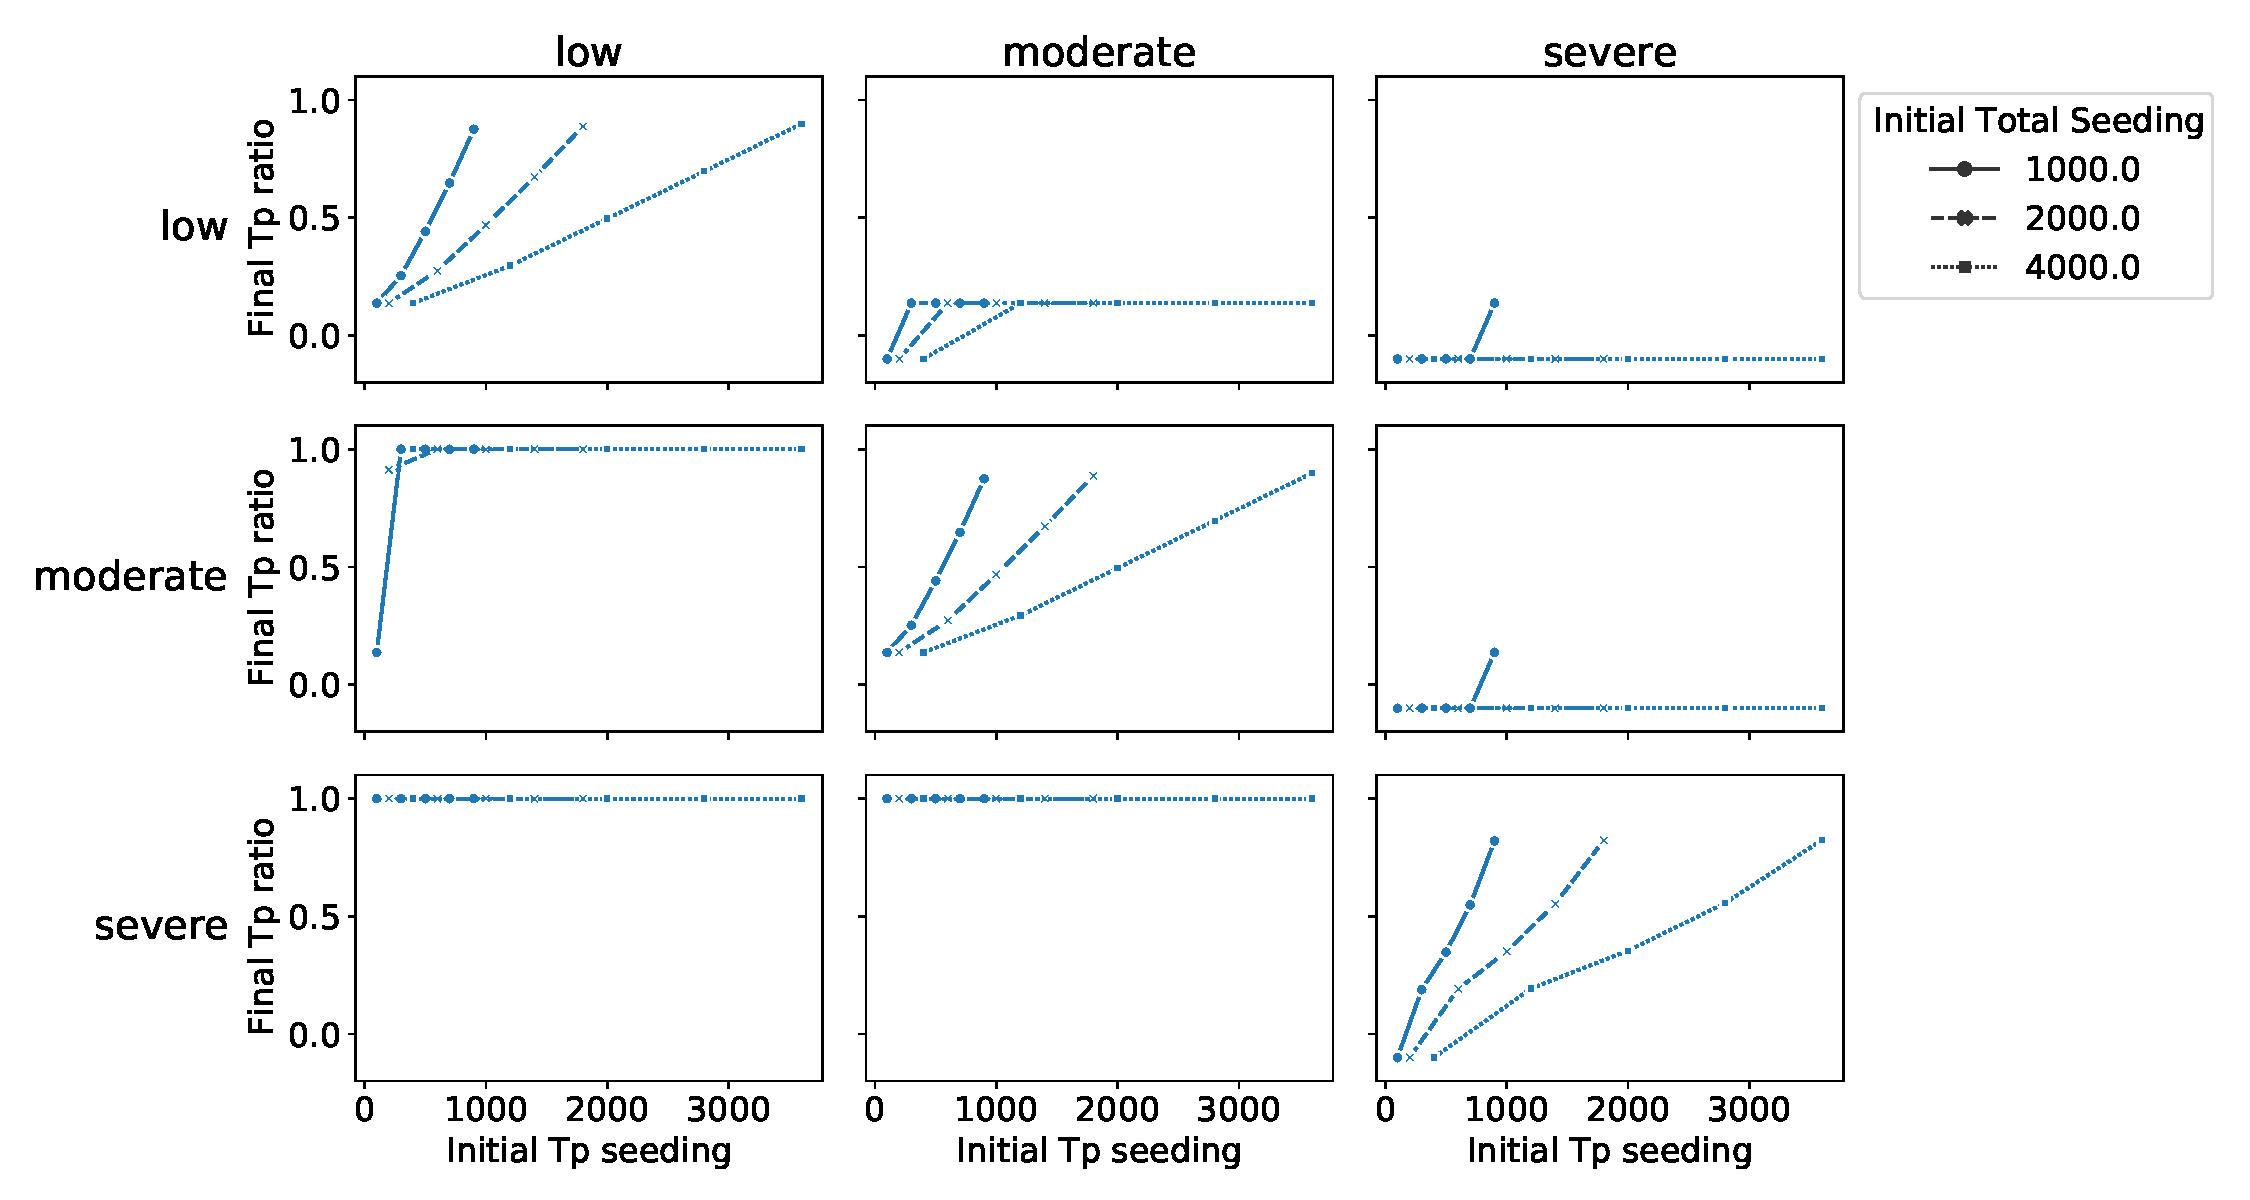
\includegraphics[width=\textwidth]{Tpos-Tpro_cases_o2}
      \caption{$O_2$ limits. C: $T^p\ O_2$ limits, R: $T^+\ O_2$ limits}
    \end{subfigure}
    \caption{Final $T^p$ ratio of pairwise $T^+ - T^p$}
  \end{figure}
  \begin{columns}
    \begin{column}{0.5\textwidth}
      \begin{itemize}
        \item Coexist: limitation same
      \end{itemize}
    \end{column}
    \begin{column}{0.5\textwidth}
      \begin{itemize}
        \item Coexist: mod.
      \end{itemize}
    \end{column}
  \end{columns}
  \framebreak
  \begin{figure}[h]\ContinuedFloat
    \centering
    \begin{subfigure}[b]{\textwidth}
      \centering
      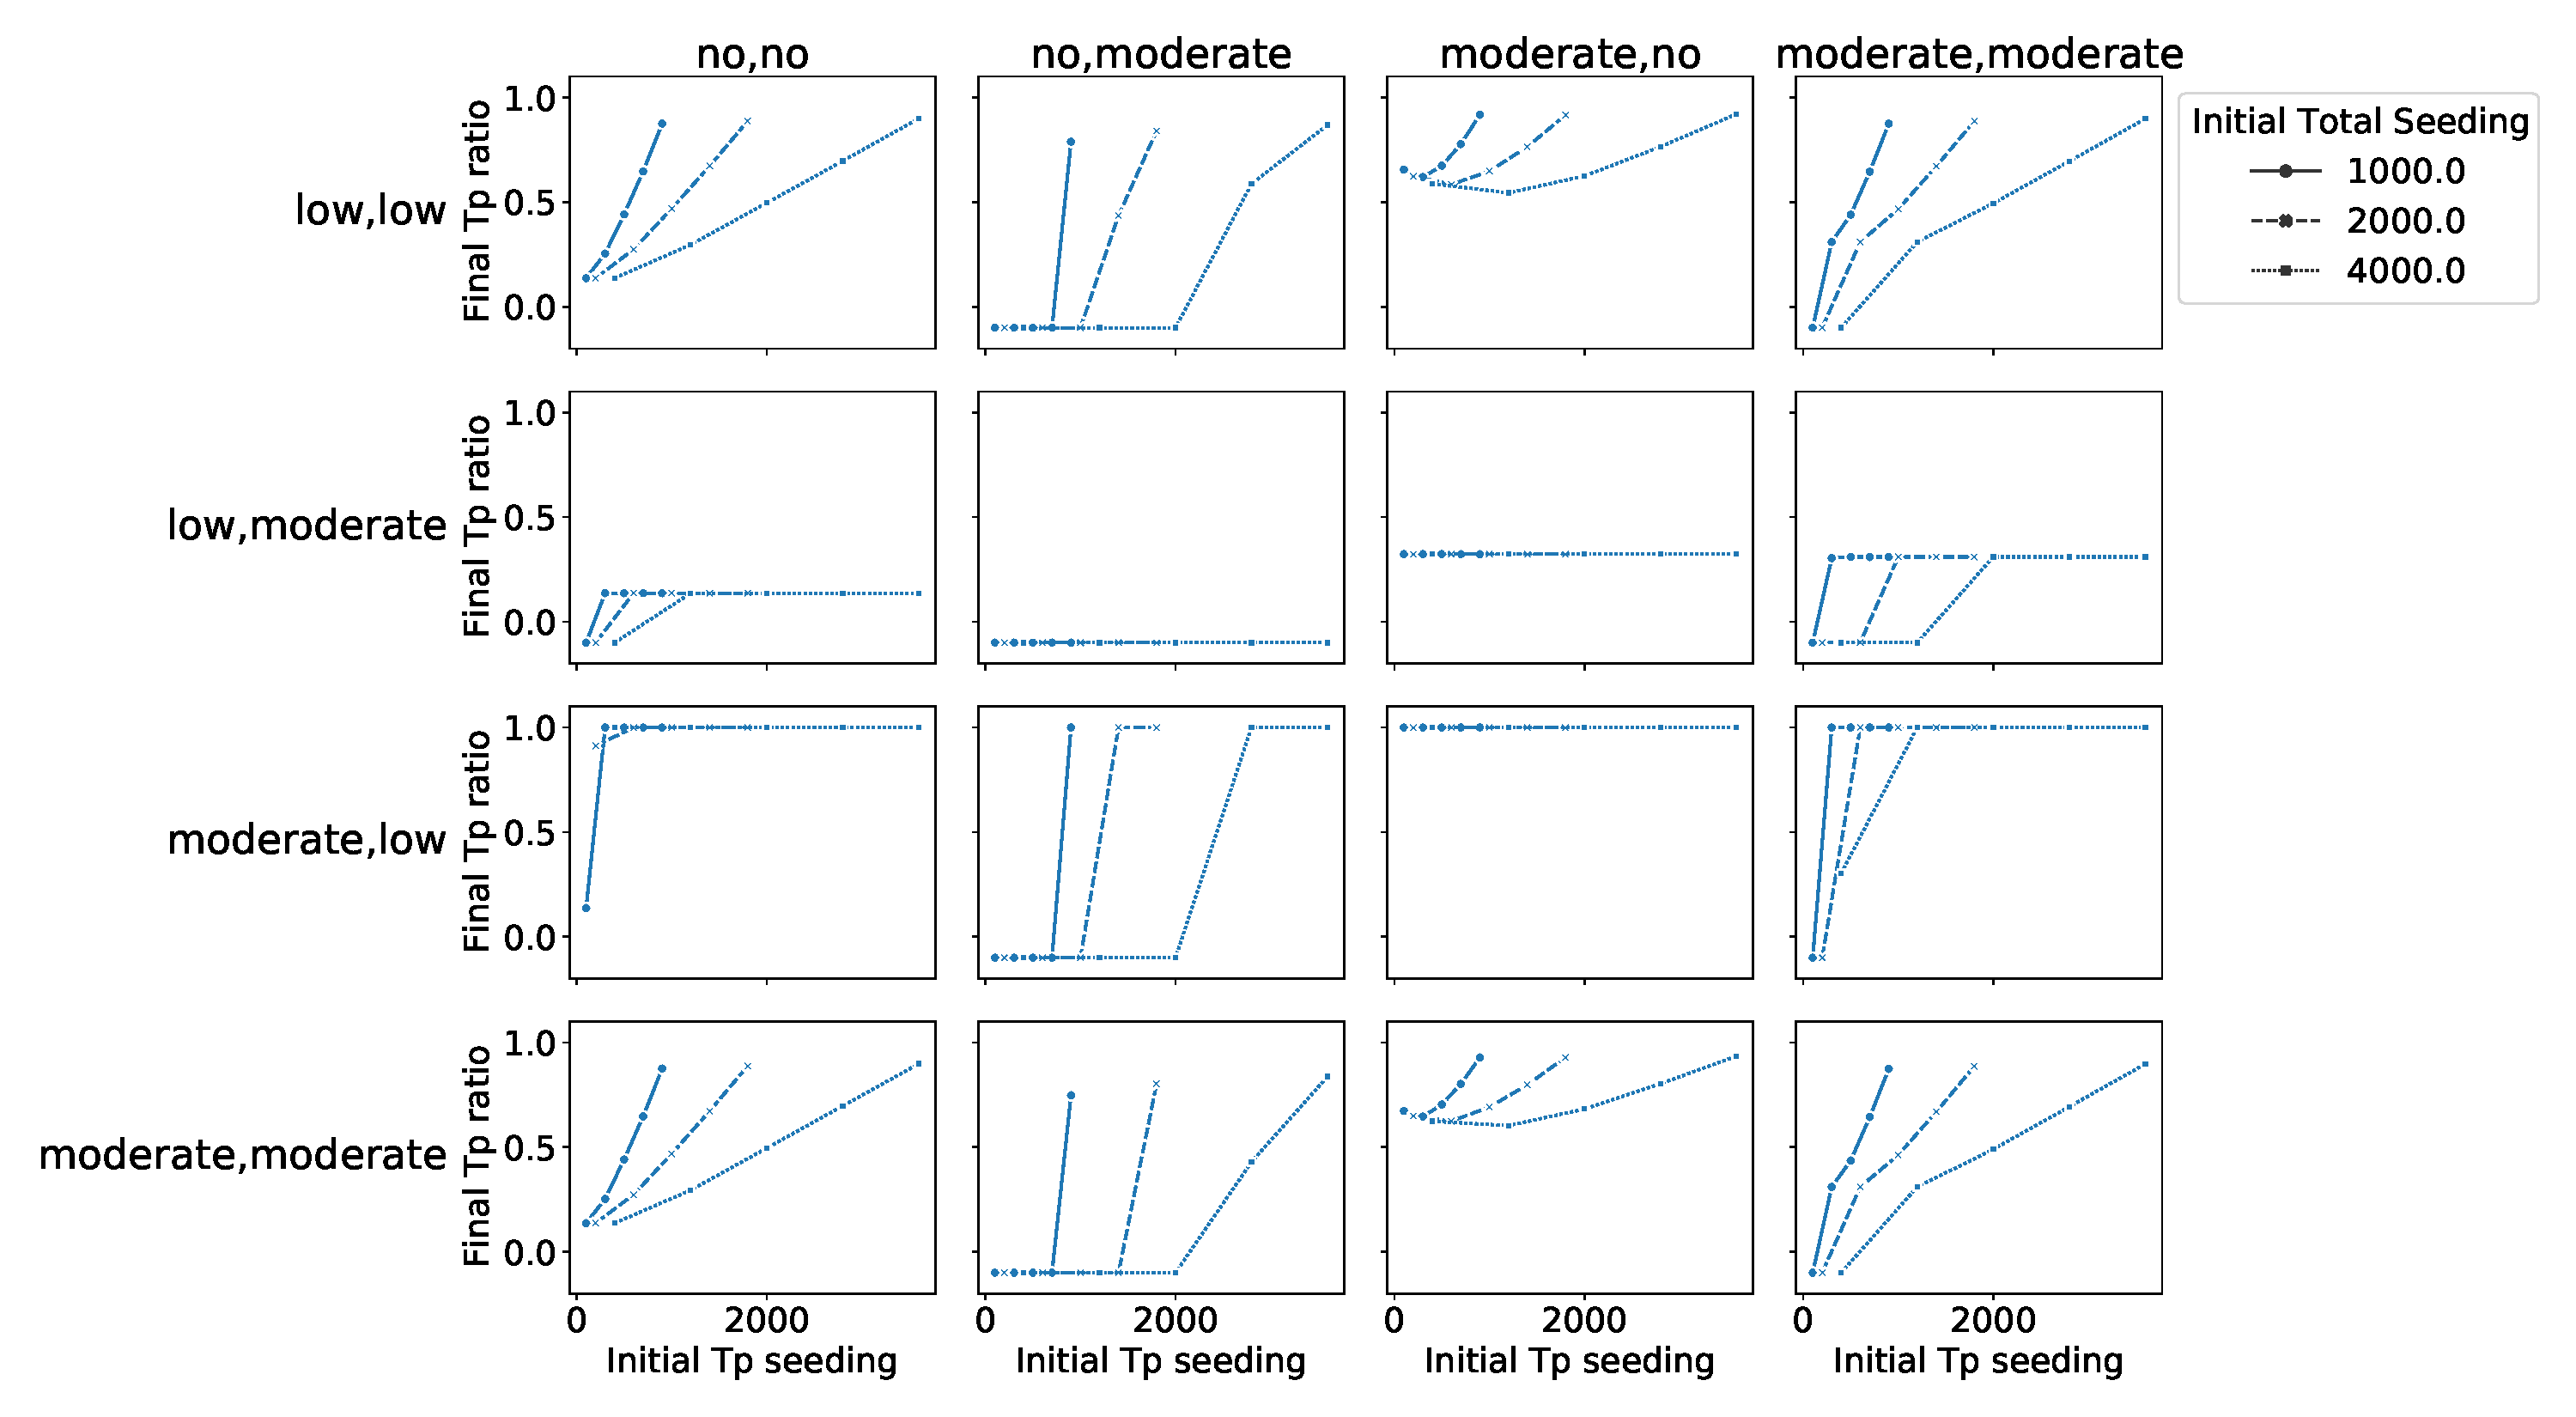
\includegraphics[width=0.5\textwidth]{Tpos-Tpro_cases}
      \caption{Combination limits. C: $T^+,T^p\ test$ limits, R: $T^+,T^p\ O_2$ limits}
    \end{subfigure}
    \caption{Final $T^p$ ratio of pairwise $T^+ - T^p$}
  \end{figure}
  \begin{itemize}
    \item Similar: symmetric limitation
  \end{itemize}
\end{frame}

\begin{frame}{All cell type cases}
  \begin{figure}[h]
    \centering
    \begin{subfigure}[b]{0.48\textwidth}
      \centering
      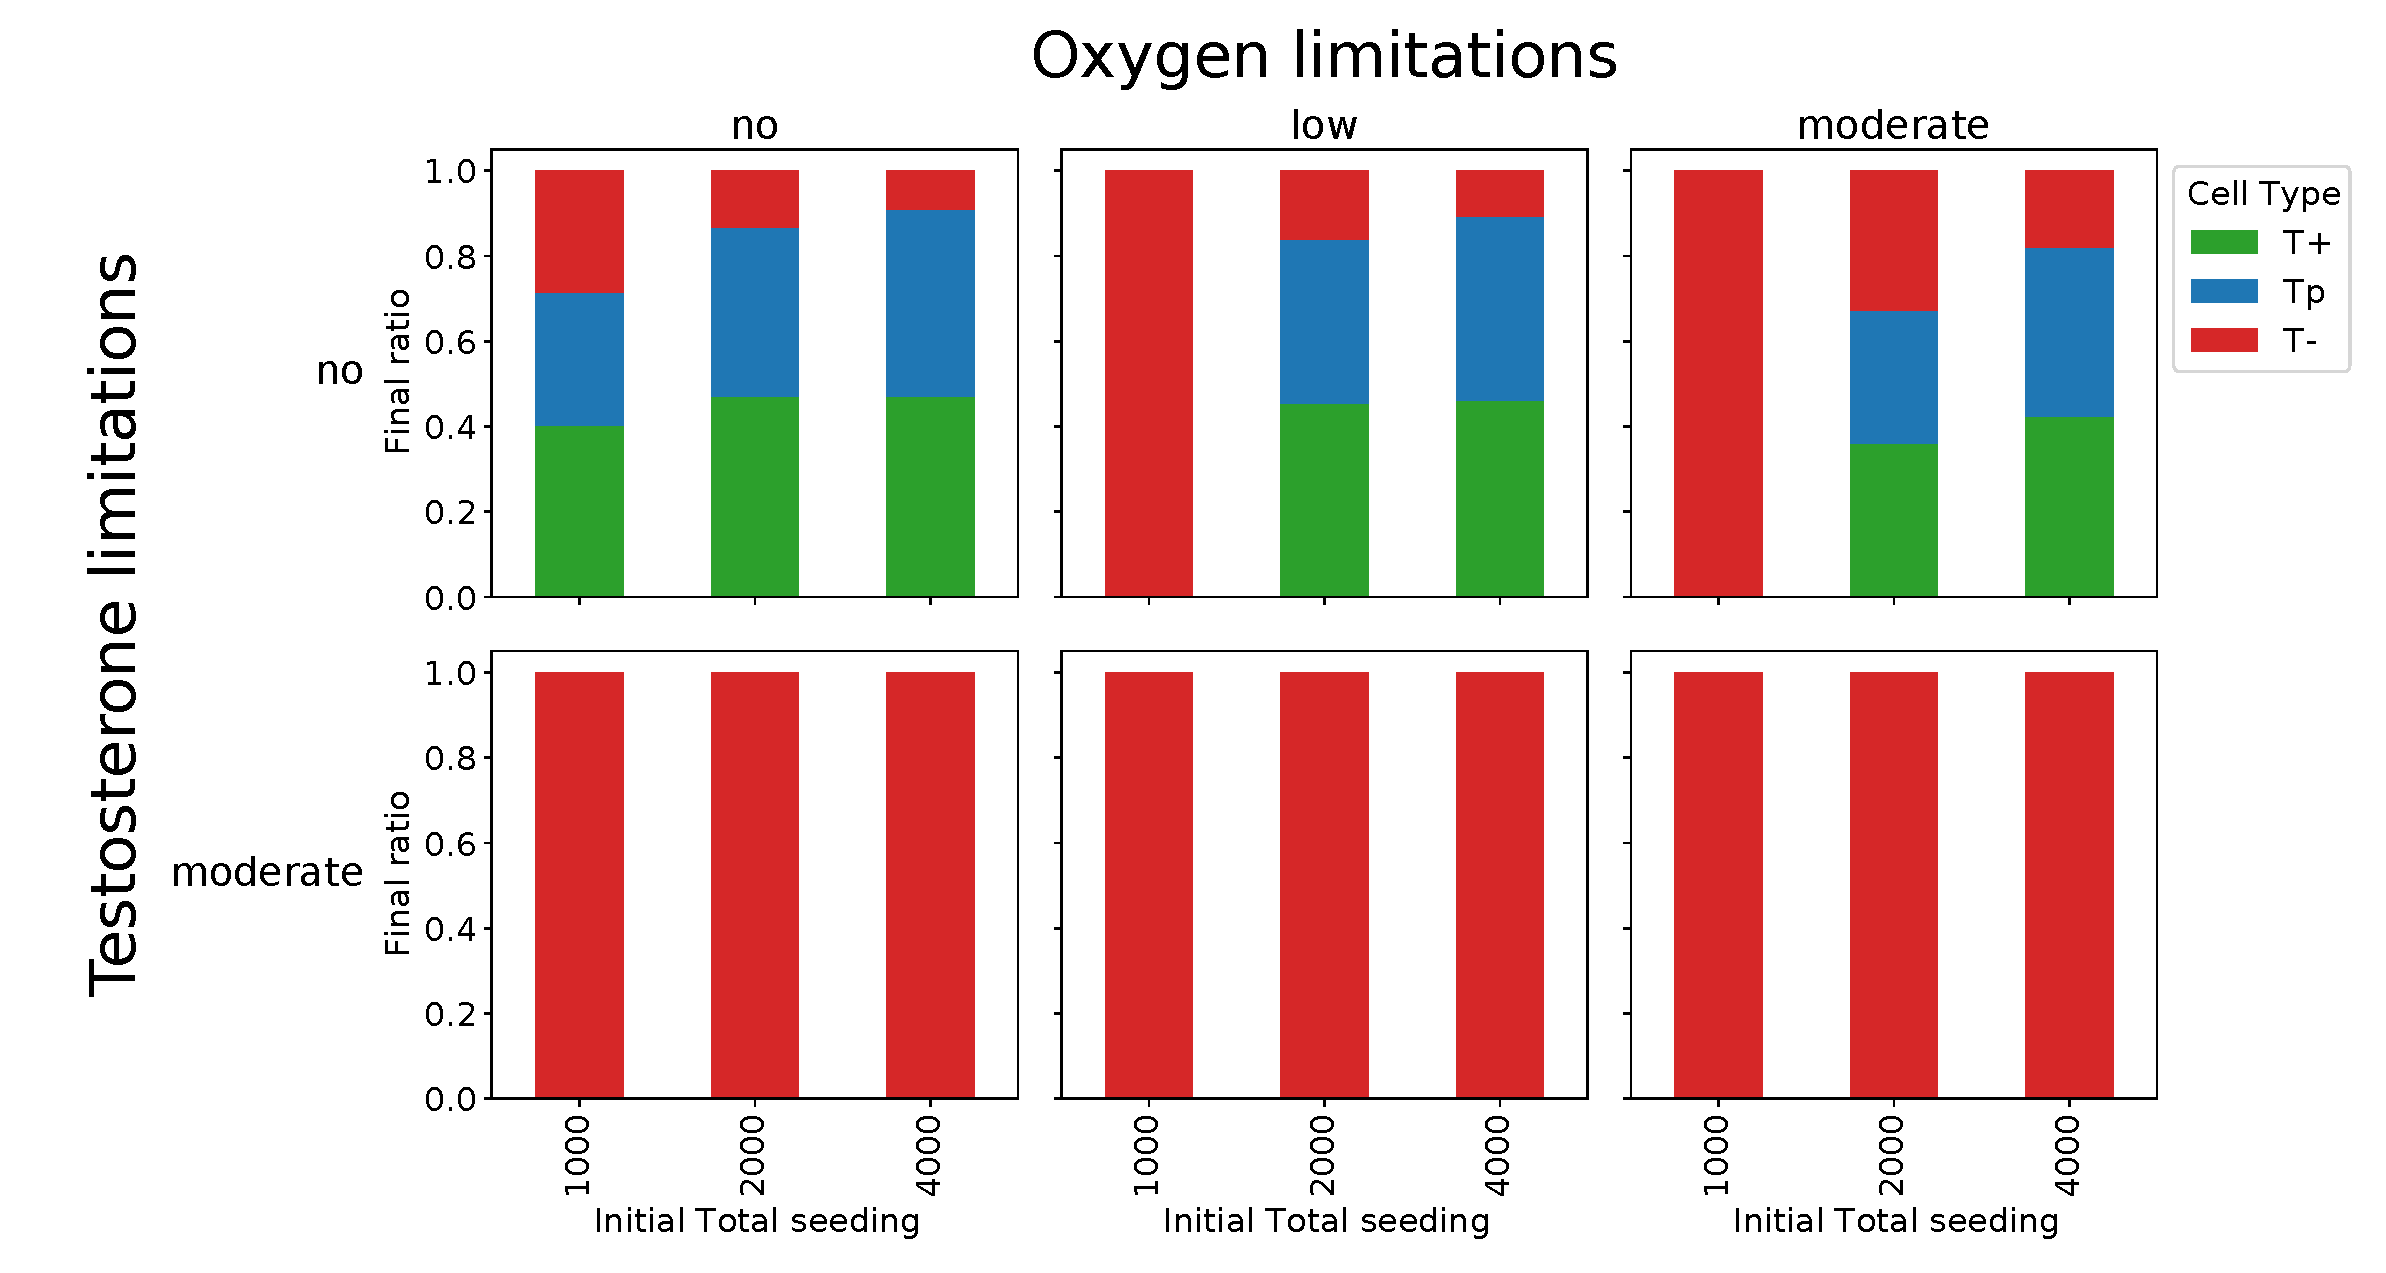
\includegraphics[width=\textwidth]{All3_efficiency_1:1:1}
      \caption{Equal seeding - 1:1:1 }
    \end{subfigure}
    \begin{subfigure}[b]{0.48\textwidth}
      \centering
      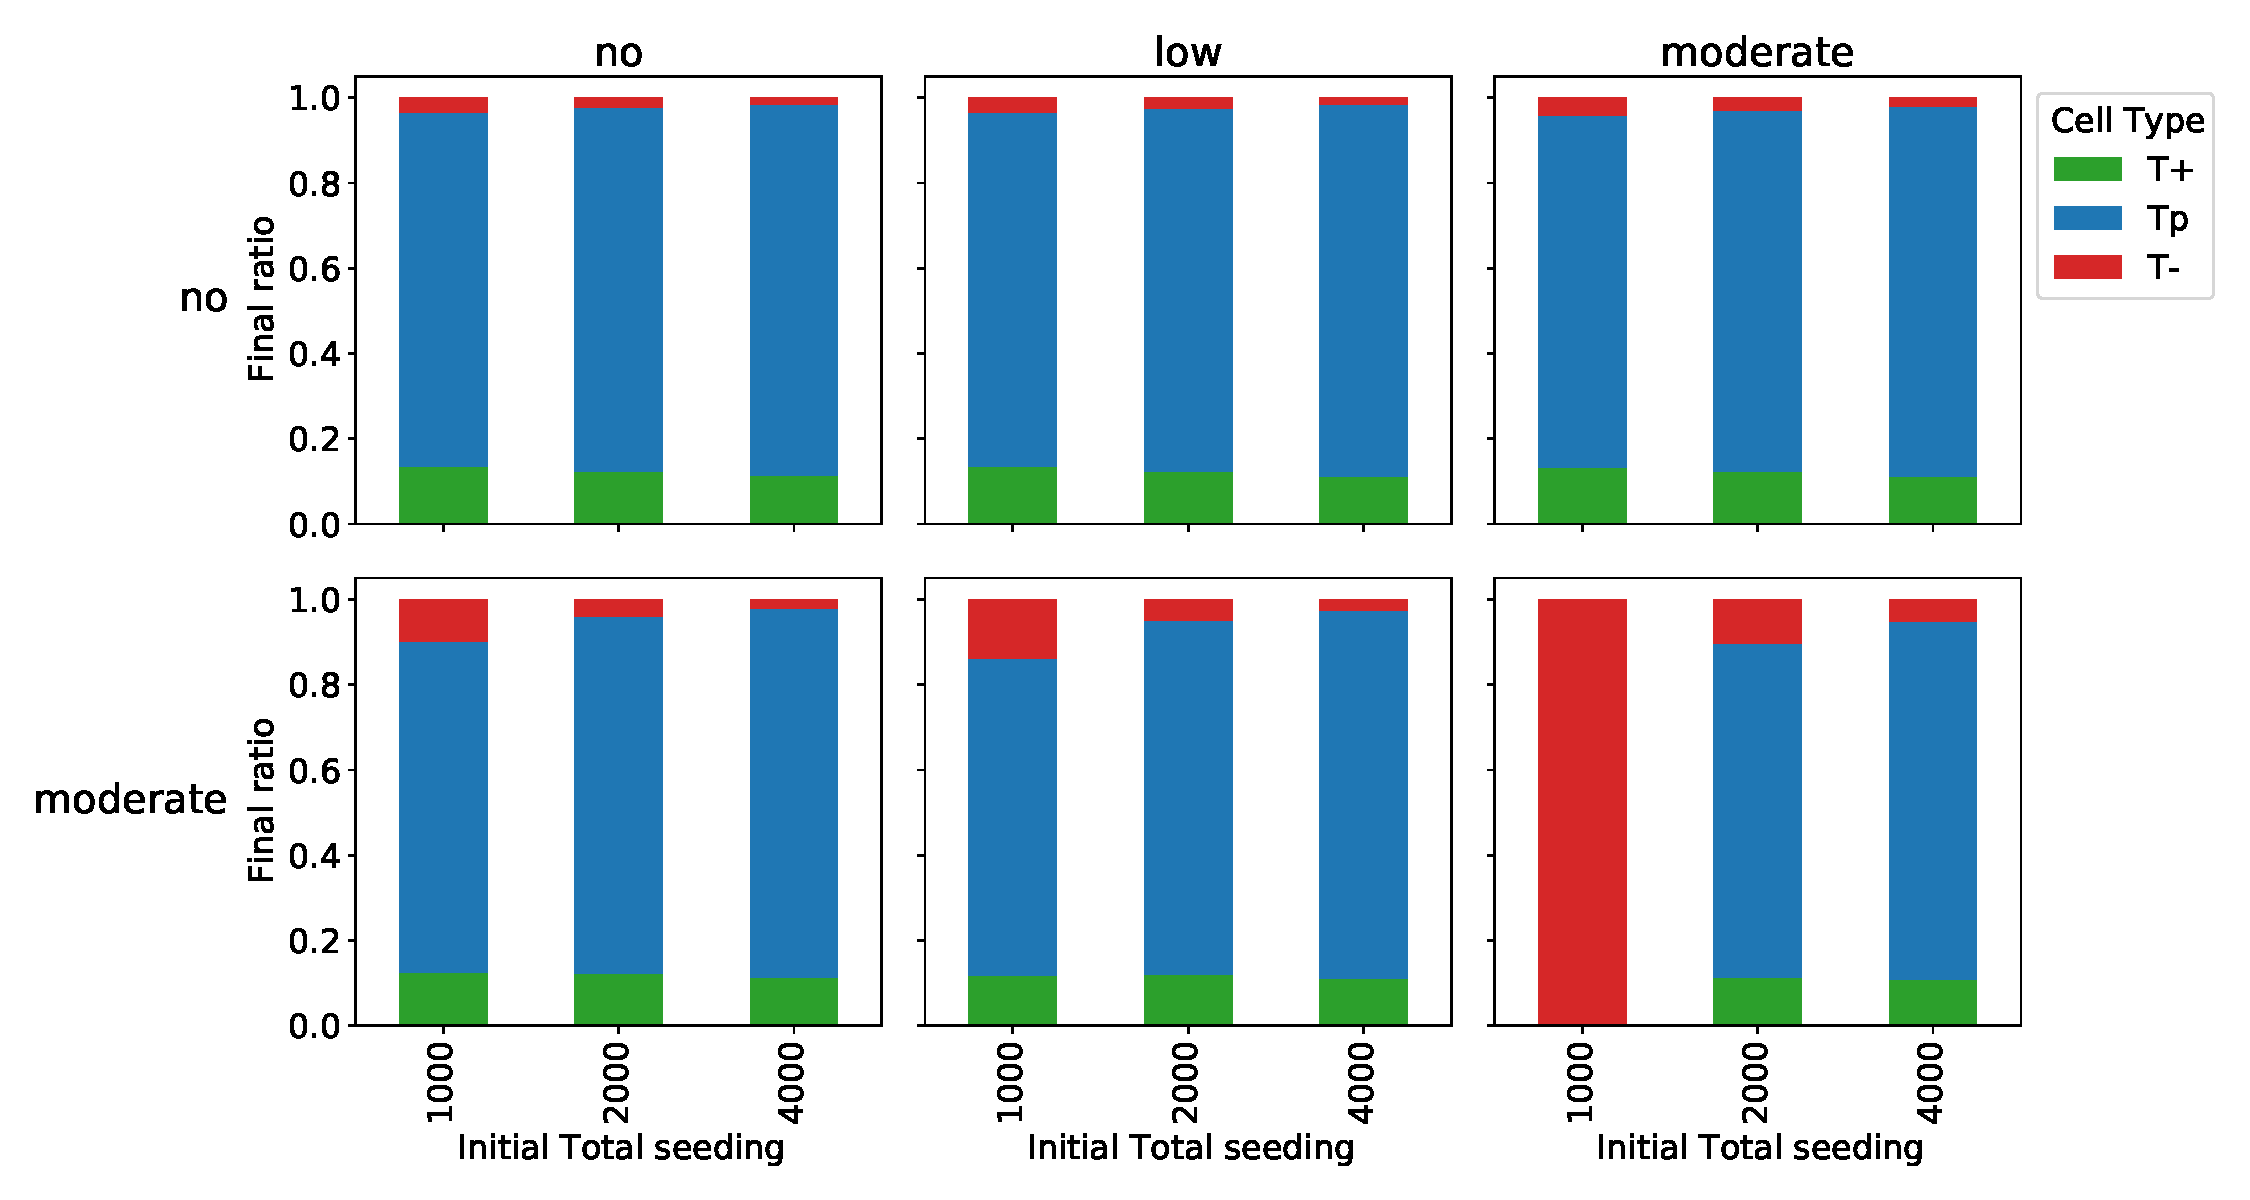
\includegraphics[width=\textwidth]{All3_efficiency_8:1:1}
      \caption{High $T^p$ seeding - 8:1:1}
    \end{subfigure}
    \caption{Final ratio of all cell types. C: $O_2$ limits , R: $test$ limits and SF: seeding propn.}
  \end{figure}
  \begin{columns}
    \begin{column}{0.5\textwidth}
      \begin{itemize}
        \item Homogenous: $test$ private resource
        \item No vs Mod: Weak vs Strong interspecific
      \end{itemize}
    \end{column}
    \begin{column}{0.5\textwidth}
      \begin{itemize}
        \item $O_2$: 3 zones of effect
      \end{itemize}
    \end{column}
  \end{columns}
\end{frame}


\section{Therapy}

\begin{frame}{Therapy Implementation}
  \begin{columns}
    \begin{column}{0.4\textwidth}
      \begin{itemize}
        \item Therapy: boolean - 1 = MTD
      \end{itemize}
      \begin{equation}
        p_{test}(abi) = \begin{cases}
        p_{test,max} &\text{if } abi = 0 \\
        p_{test,min} &\text{if } abi = 1 \\
        \end{cases}
        \label{p_test_dose_eq}
      \end{equation}
      \begin{equation}
        r_i(dtx) = \begin{cases}
        r_{i,max} &\text{if } dtx = 0 \\
        r_{i,min} &\text{if } dtx = 1 \\
        \end{cases}
        \label{r_dose_eq}
      \end{equation}
    \end{column}
    \begin{column}{0.6\textwidth}
      \begin{itemize}
        \item SOC: dose at MTD from start
        \begin{equation}
          dose(x,t) = 1 \quad \forall\ t, x
          \label{dose_soc_eq}
        \end{equation}
        \item AT: binary mode, switch on/off therapy
        \begin{equation}
          dose(x,t) = \begin{cases}
          0 &\text{if } dose(x,t-\Delta t) = 0 \text{ and } x < \text{On} \\
          1 &\text{if } dose(x,t-\Delta t) = 0 \text{ and } x \geq \text{On} \\
          1 &\text{if } dose(x,t-\Delta t) = 1 \text{ and } x > \text{Off} \\
          0 &\text{if } dose(x,t-\Delta t) = 1 \text{ and } x \leq \text{Off} \\
          \end{cases}
          \label{dose_at_eq}
        \end{equation}
      \end{itemize}
    \end{column}
  \end{columns}
\end{frame}

\begin{frame}{Standard of care (SOC)}
  \begin{figure}[h]
    \centering
    \begin{subfigure}[b]{0.48\textwidth}
      \centering
      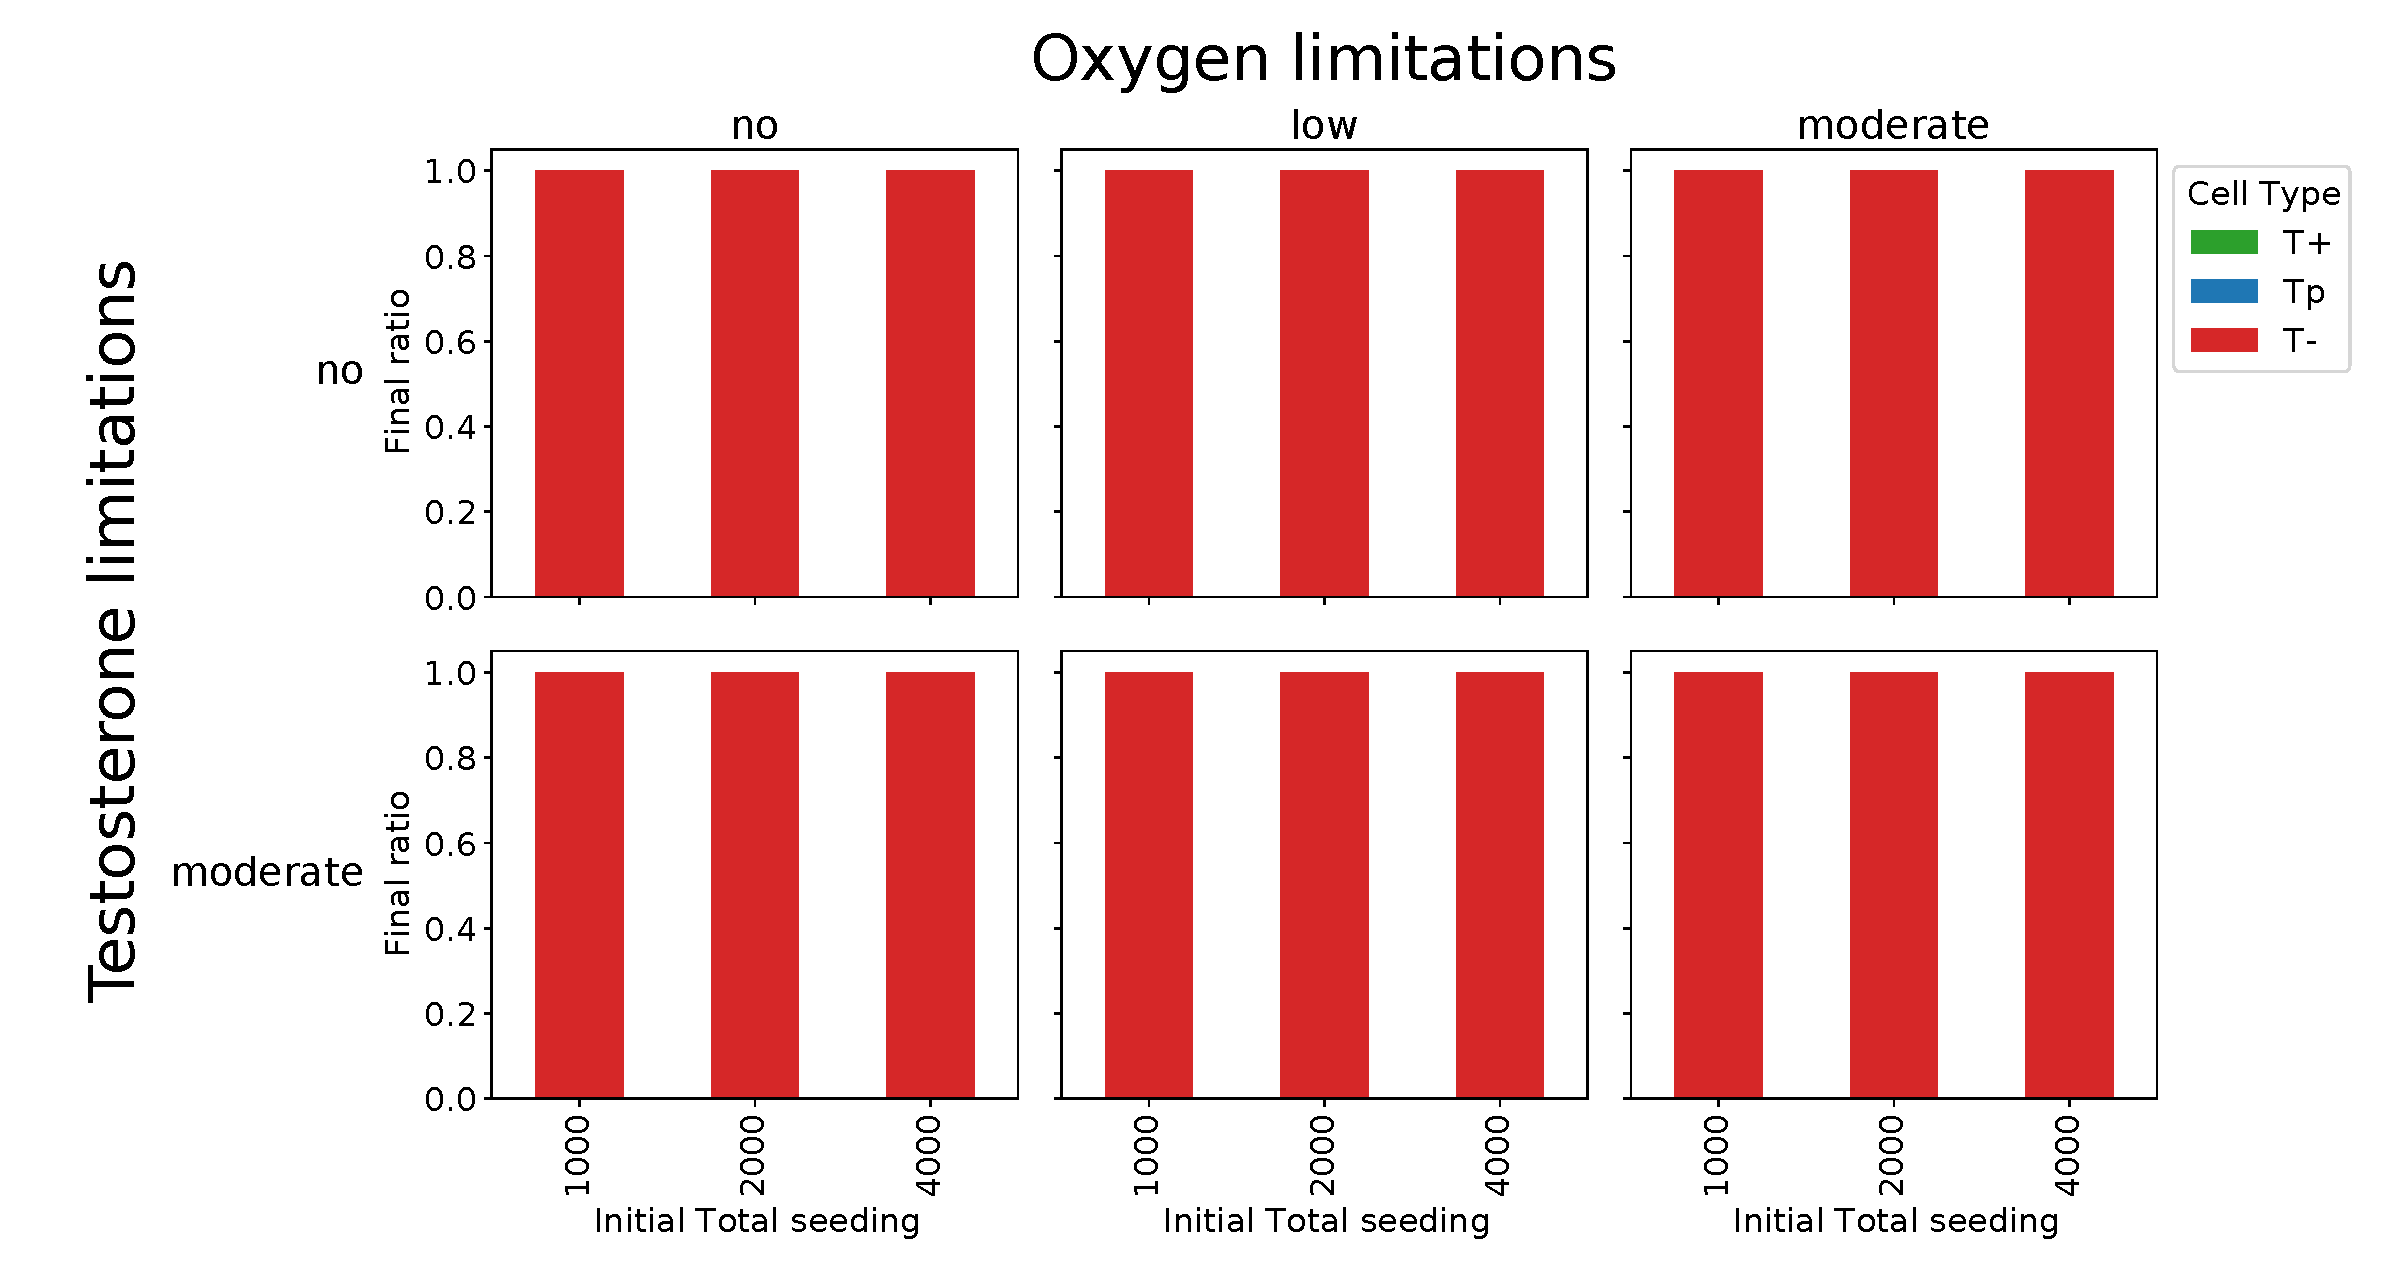
\includegraphics[width=\textwidth]{All3_therapy-SOC_1:1:1}
      \caption{Equal seeding - 1:1:1}
    \end{subfigure}
    \begin{subfigure}[b]{0.48\textwidth}
      \centering
      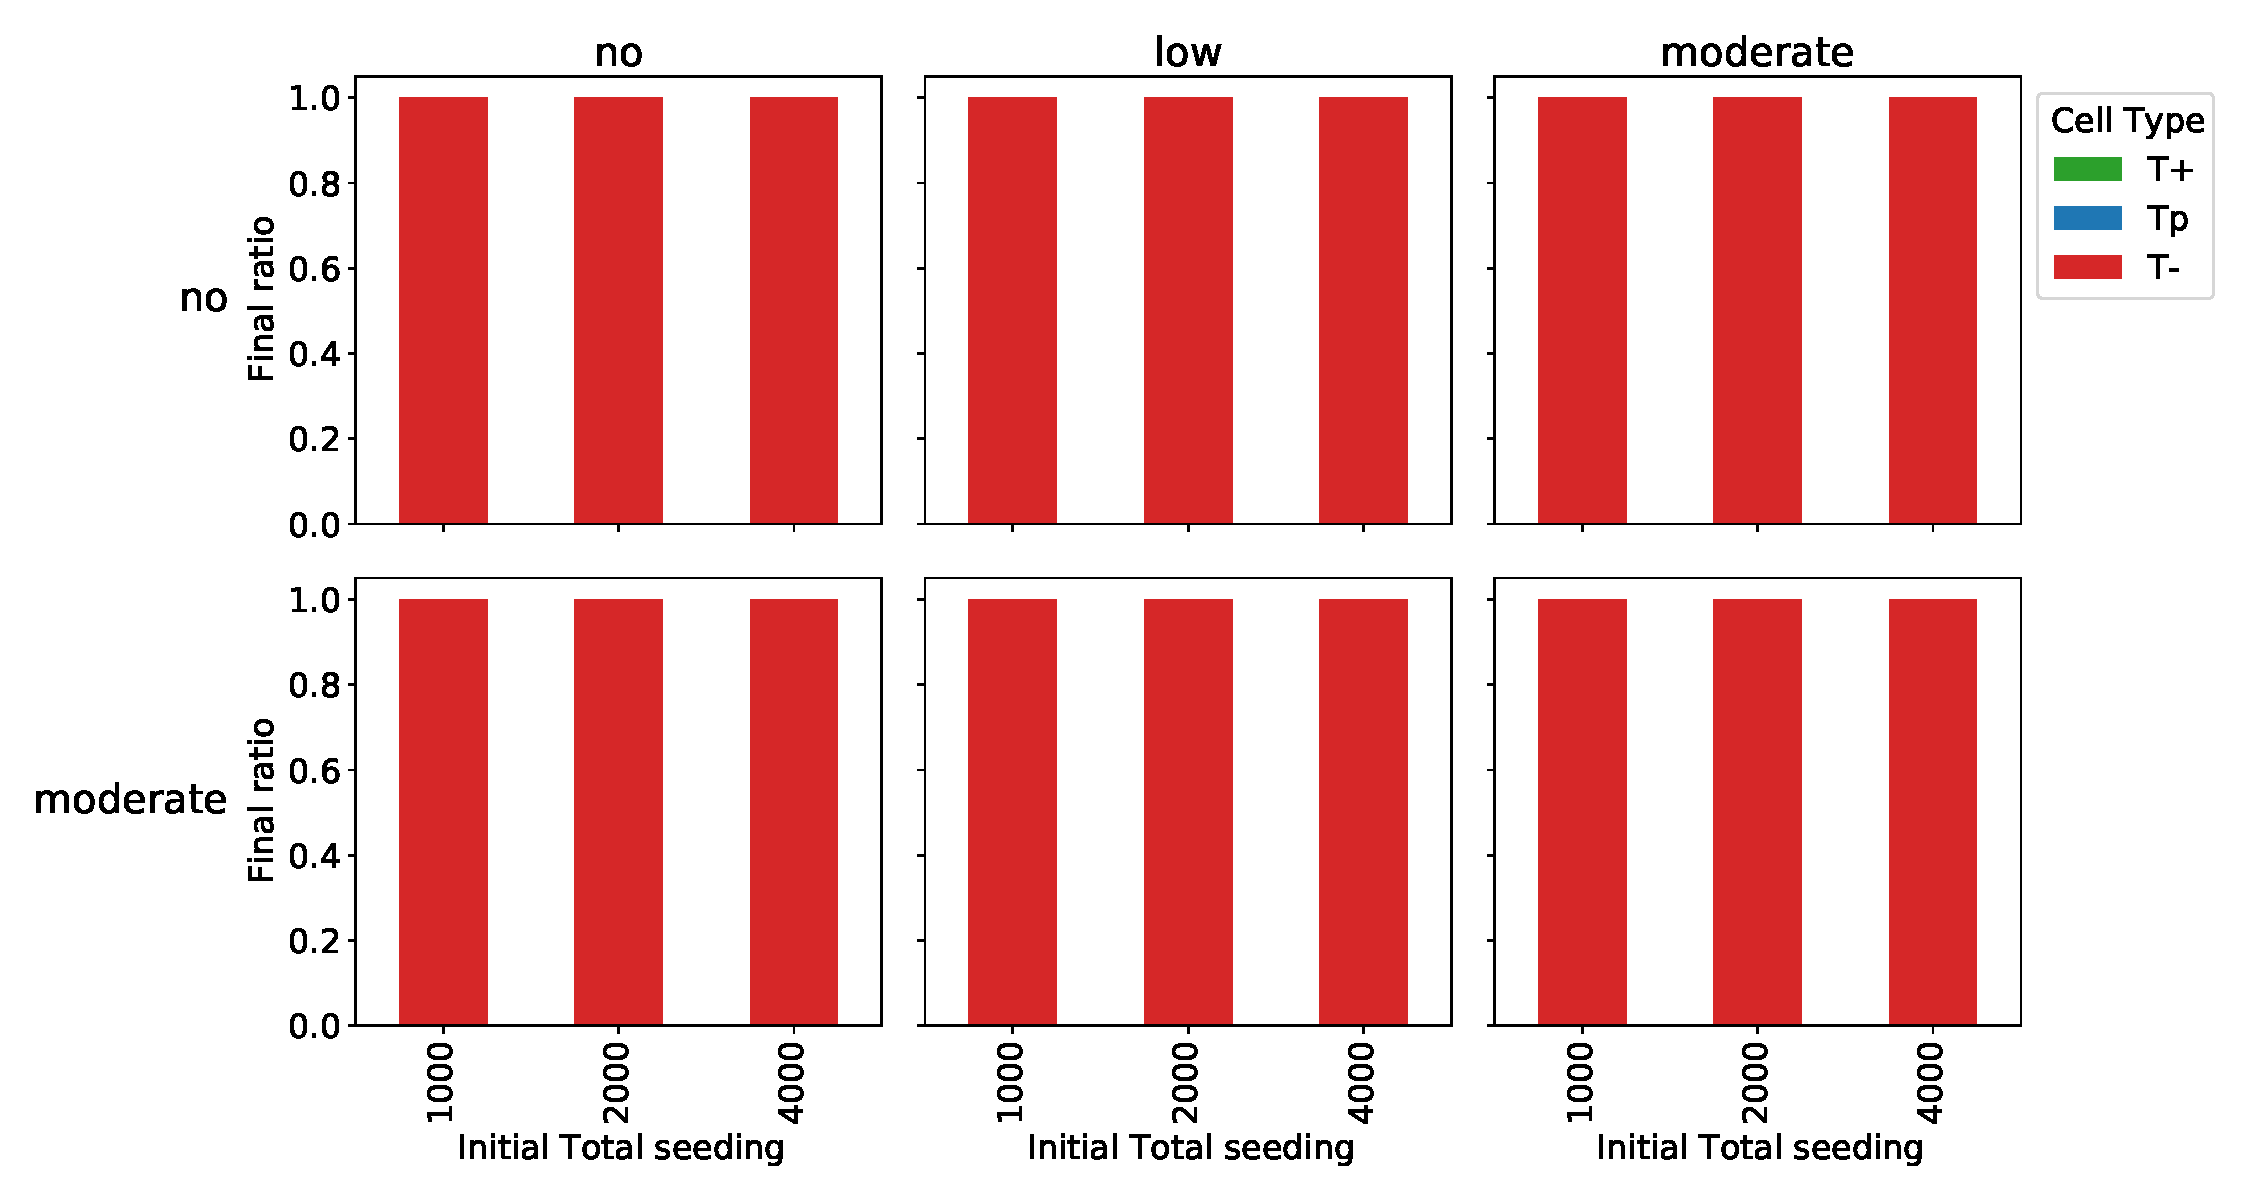
\includegraphics[width=\textwidth]{All3_therapy-SOC_8:1:1}
      \caption{High $T^p$ seeding - 8:1:1}
    \end{subfigure}
    \caption{Final ratio of all cell types under standard-of-care. C: $O_2$ limits , R: $test$ limits and SF: seeding propn. }
  \end{figure}
  \begin{columns}
    \begin{column}{0.5\textwidth}
      \begin{itemize}
        \item $T^+, T^p$ extinct: all cases
      \end{itemize}
    \end{column}
    \begin{column}{0.5\textwidth}
      \begin{itemize}
        \item $test$: insufficient
      \end{itemize}
    \end{column}
  \end{columns}
\end{frame}

\begin{frame}{Adaptive Therapy (AT) thresholds}
  \begin{figure}[h]
    \centering
    \begin{subfigure}[b]{0.48\textwidth}
      \centering
      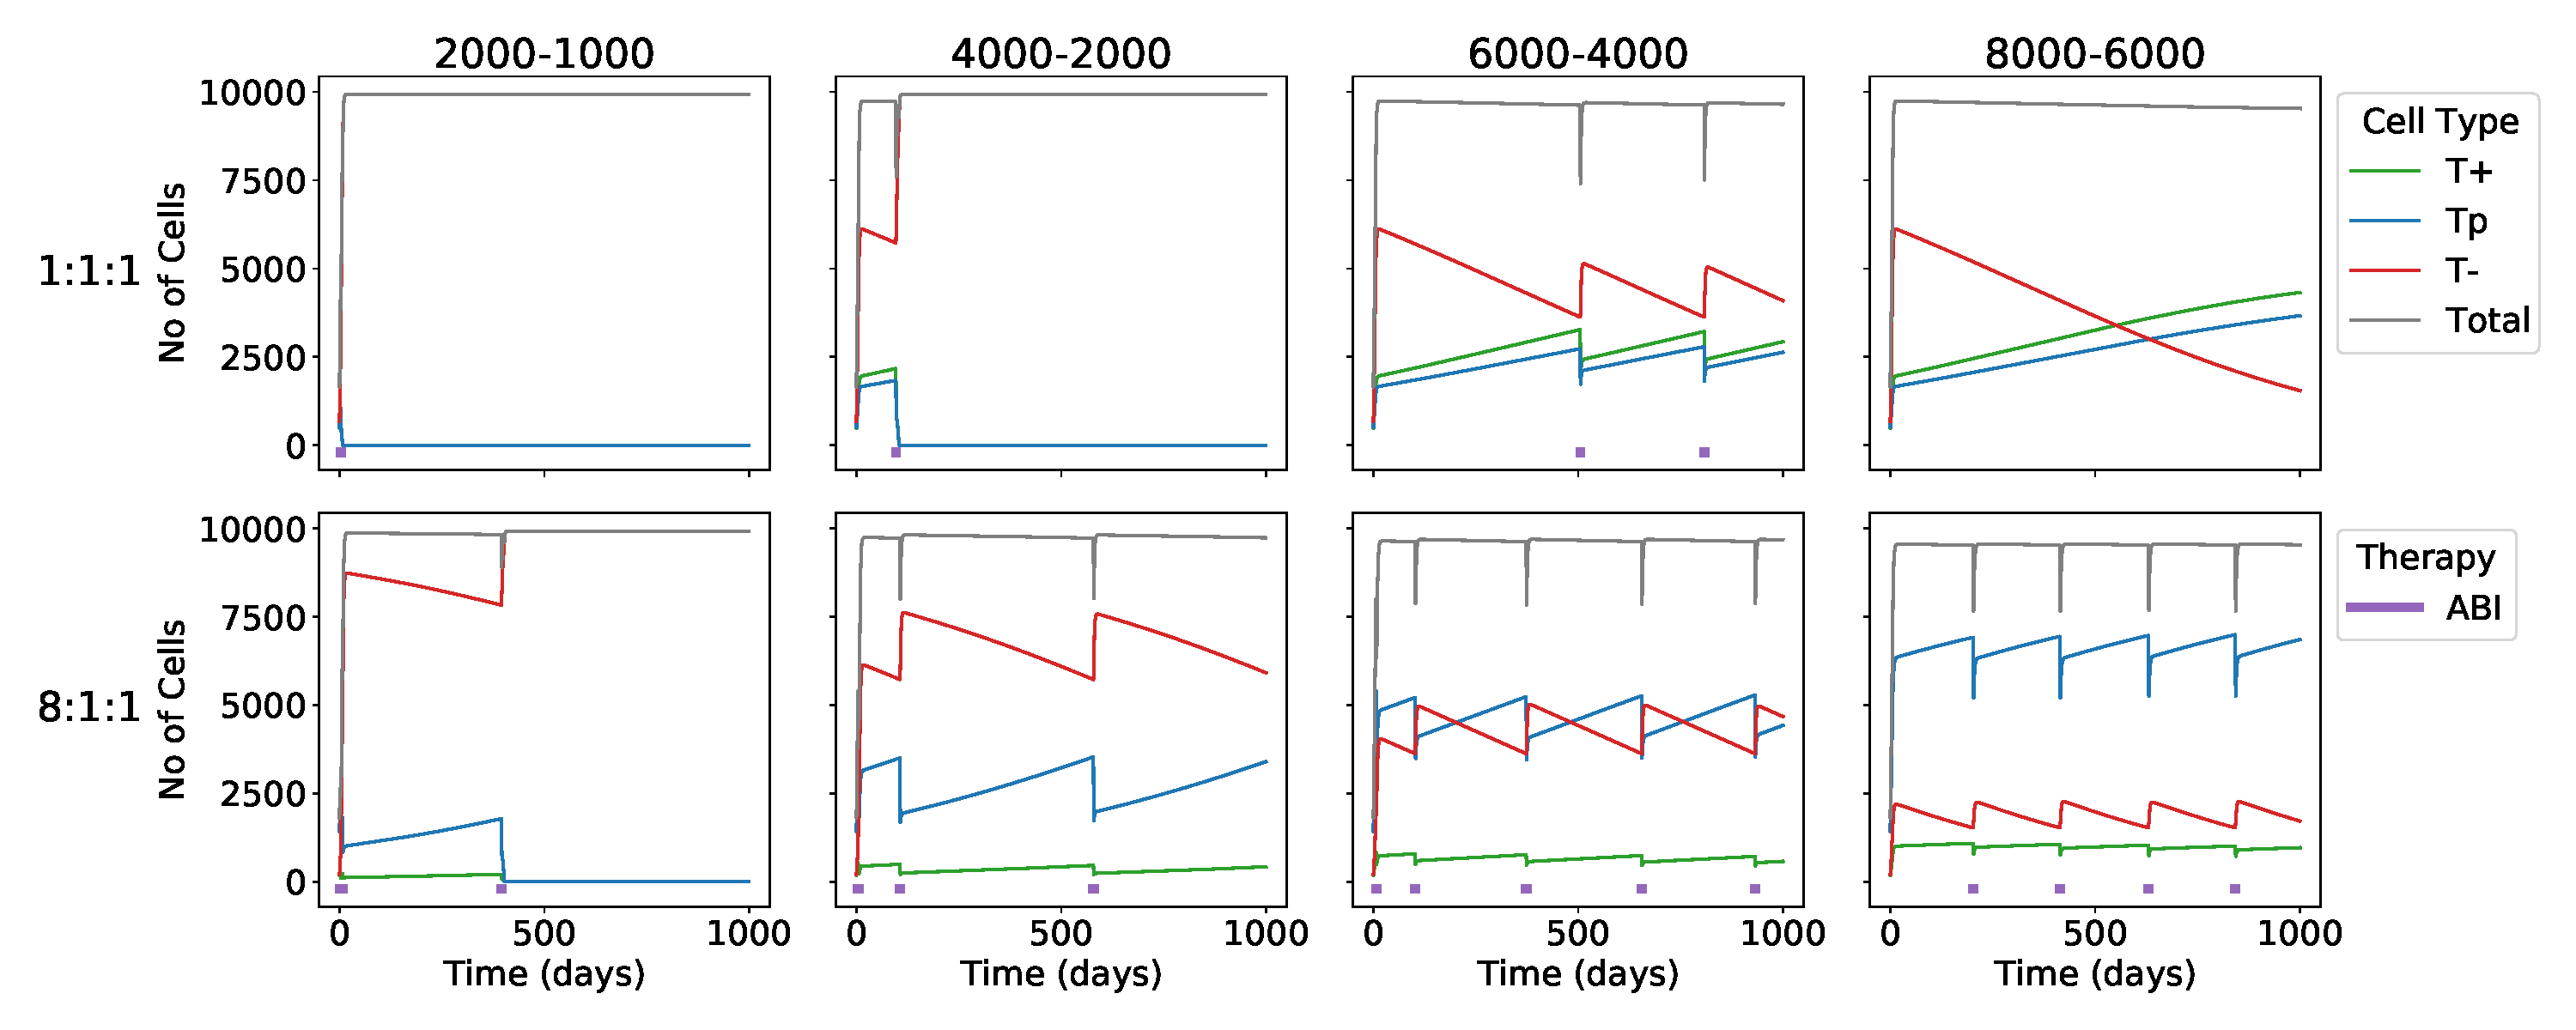
\includegraphics[width=\textwidth]{All3_therapy-standardization}
    \end{subfigure}
    \begin{subfigure}[b]{0.48\textwidth}
      \centering
      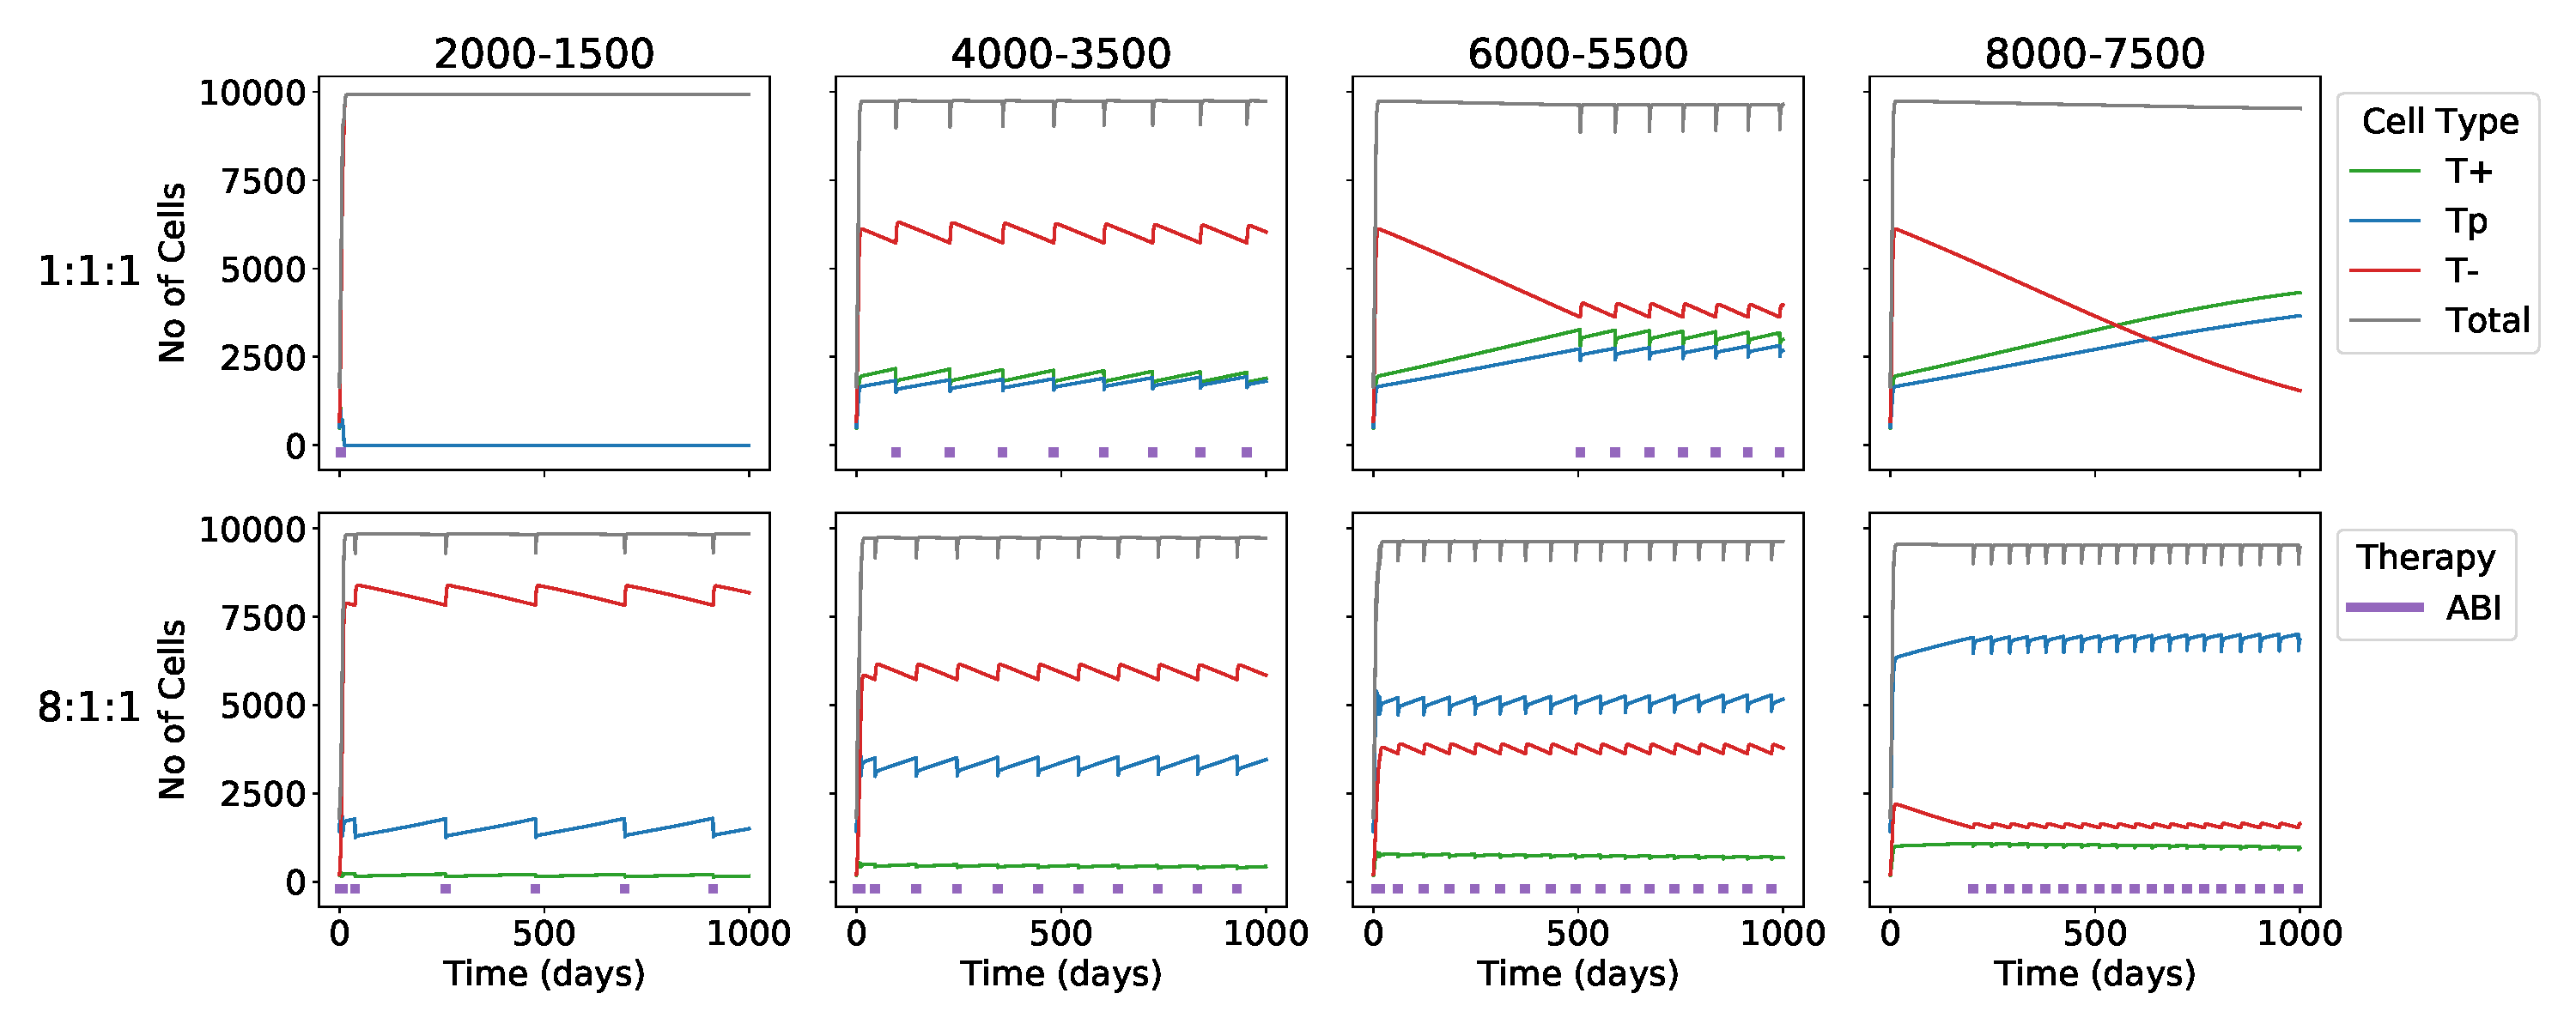
\includegraphics[width=\textwidth]{All3_therapy-standardization-sw}
    \end{subfigure}
    \caption{Standardisation of threshold for AT, C: On-Off threshold, R: $T^p:T^+:T^-$ Seeding}
  \end{figure}
  \begin{columns}
    \begin{column}{0.5\textwidth}
      \begin{itemize}
        \item $50\%$ rule
        \item Low threshold: $T^-$ inhibits
        \item High threshold: better \cite{Hansen}
      \end{itemize}
    \end{column}
    \begin{column}{0.5\textwidth}
      \begin{itemize}
        \item Too high: no therapy
        \item On: 6000, Off: 4000
        \item Popn. size $T^+ - T^p$
      \end{itemize}
    \end{column}
  \end{columns}
\end{frame}

\begin{frame}{AT}
  \begin{figure}[h]
    \centering
    \begin{subfigure}[b]{0.48\textwidth}
      \centering
      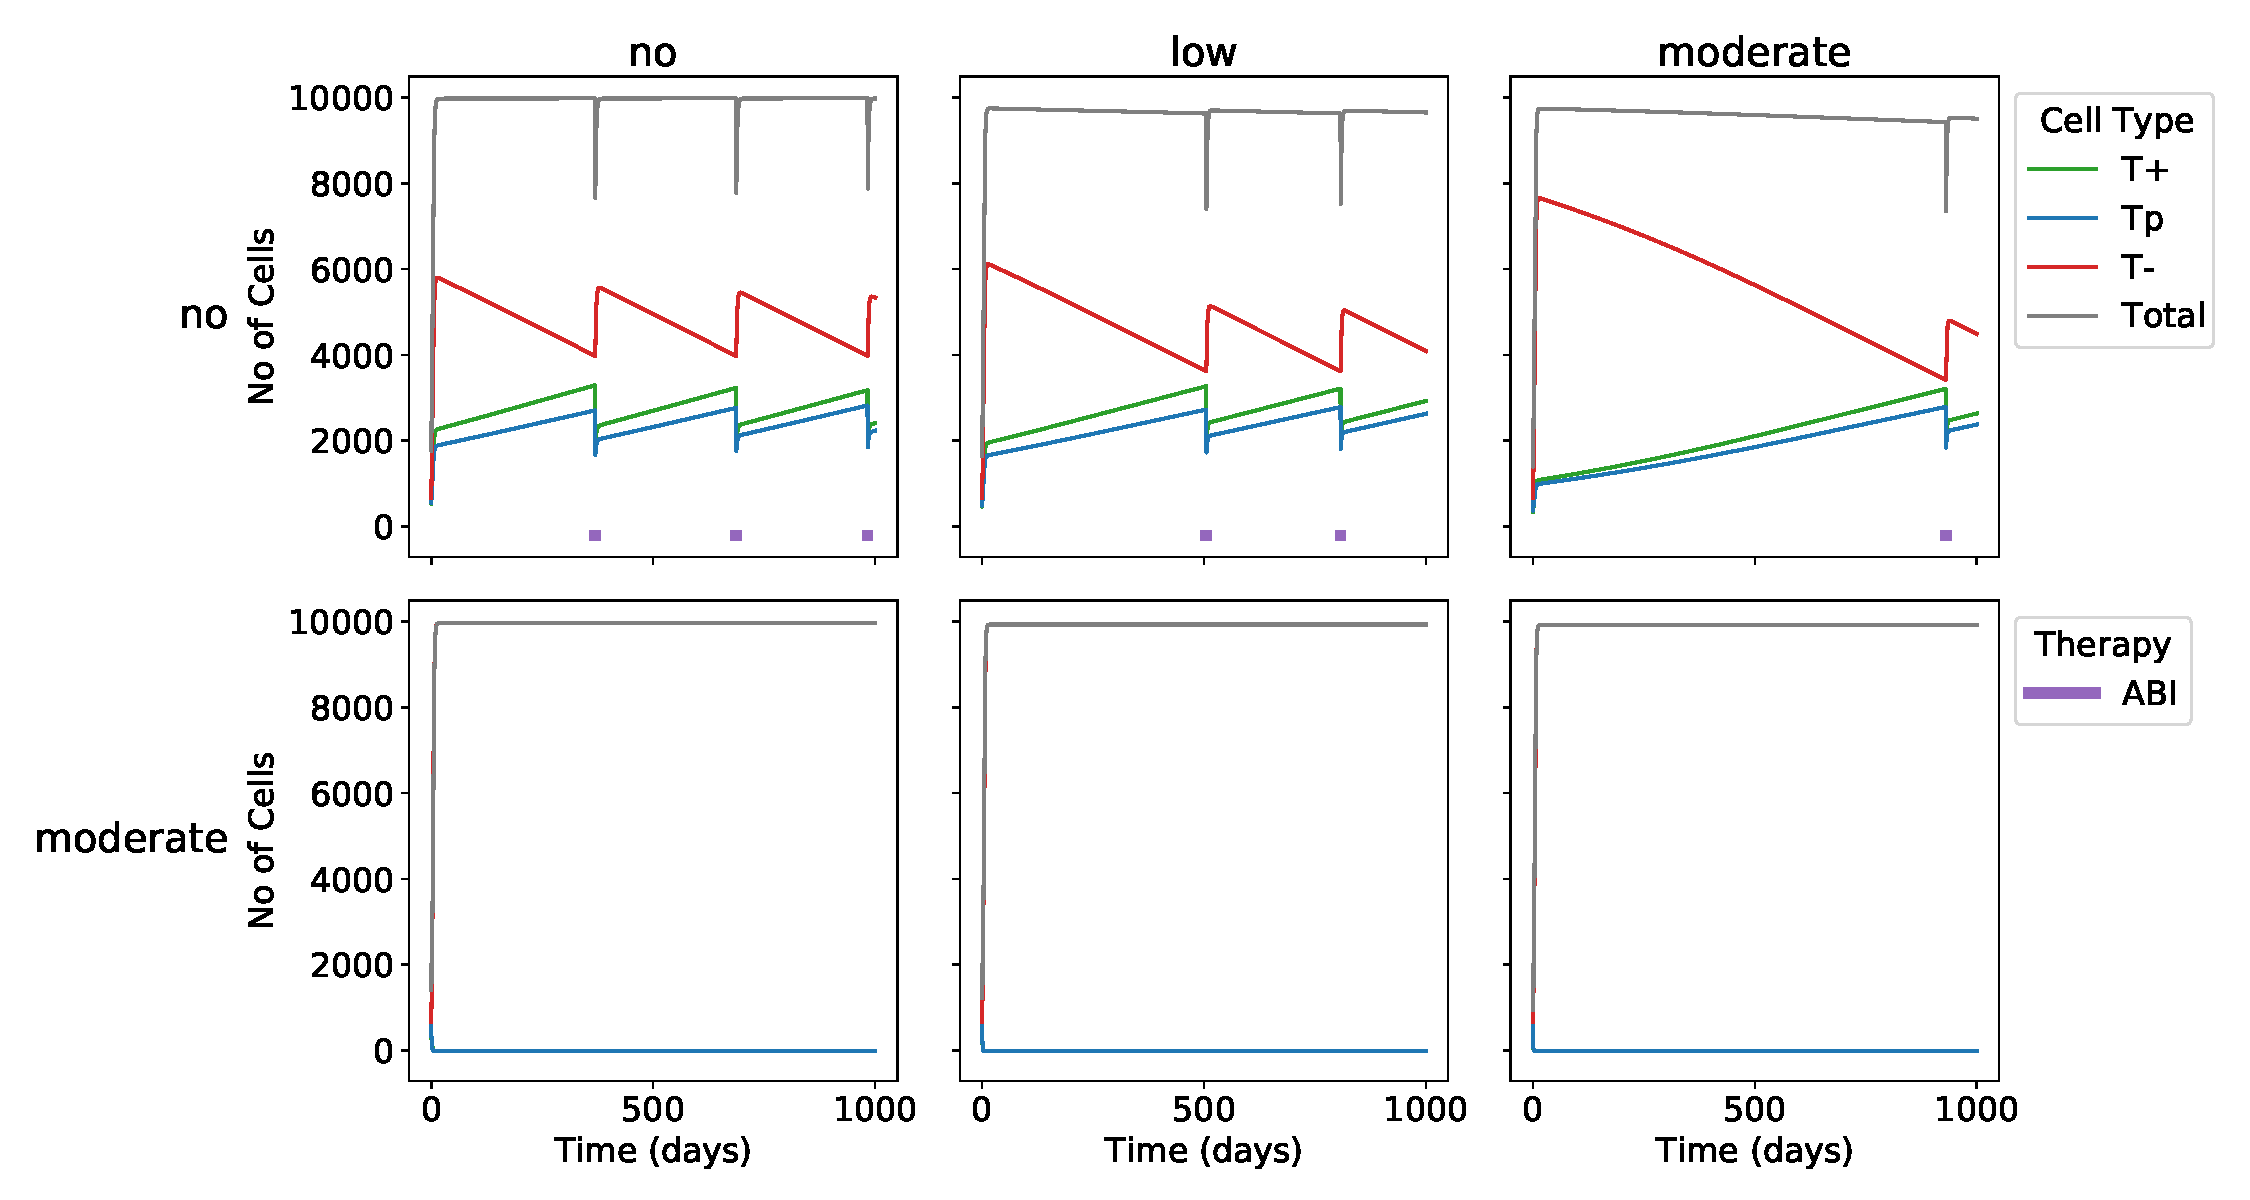
\includegraphics[width=\textwidth]{All3_therapy_1:1:1-2000}
      \caption{Equal seeding - 1:1:1}
    \end{subfigure}
    \begin{subfigure}[b]{0.48\textwidth}
      \centering
      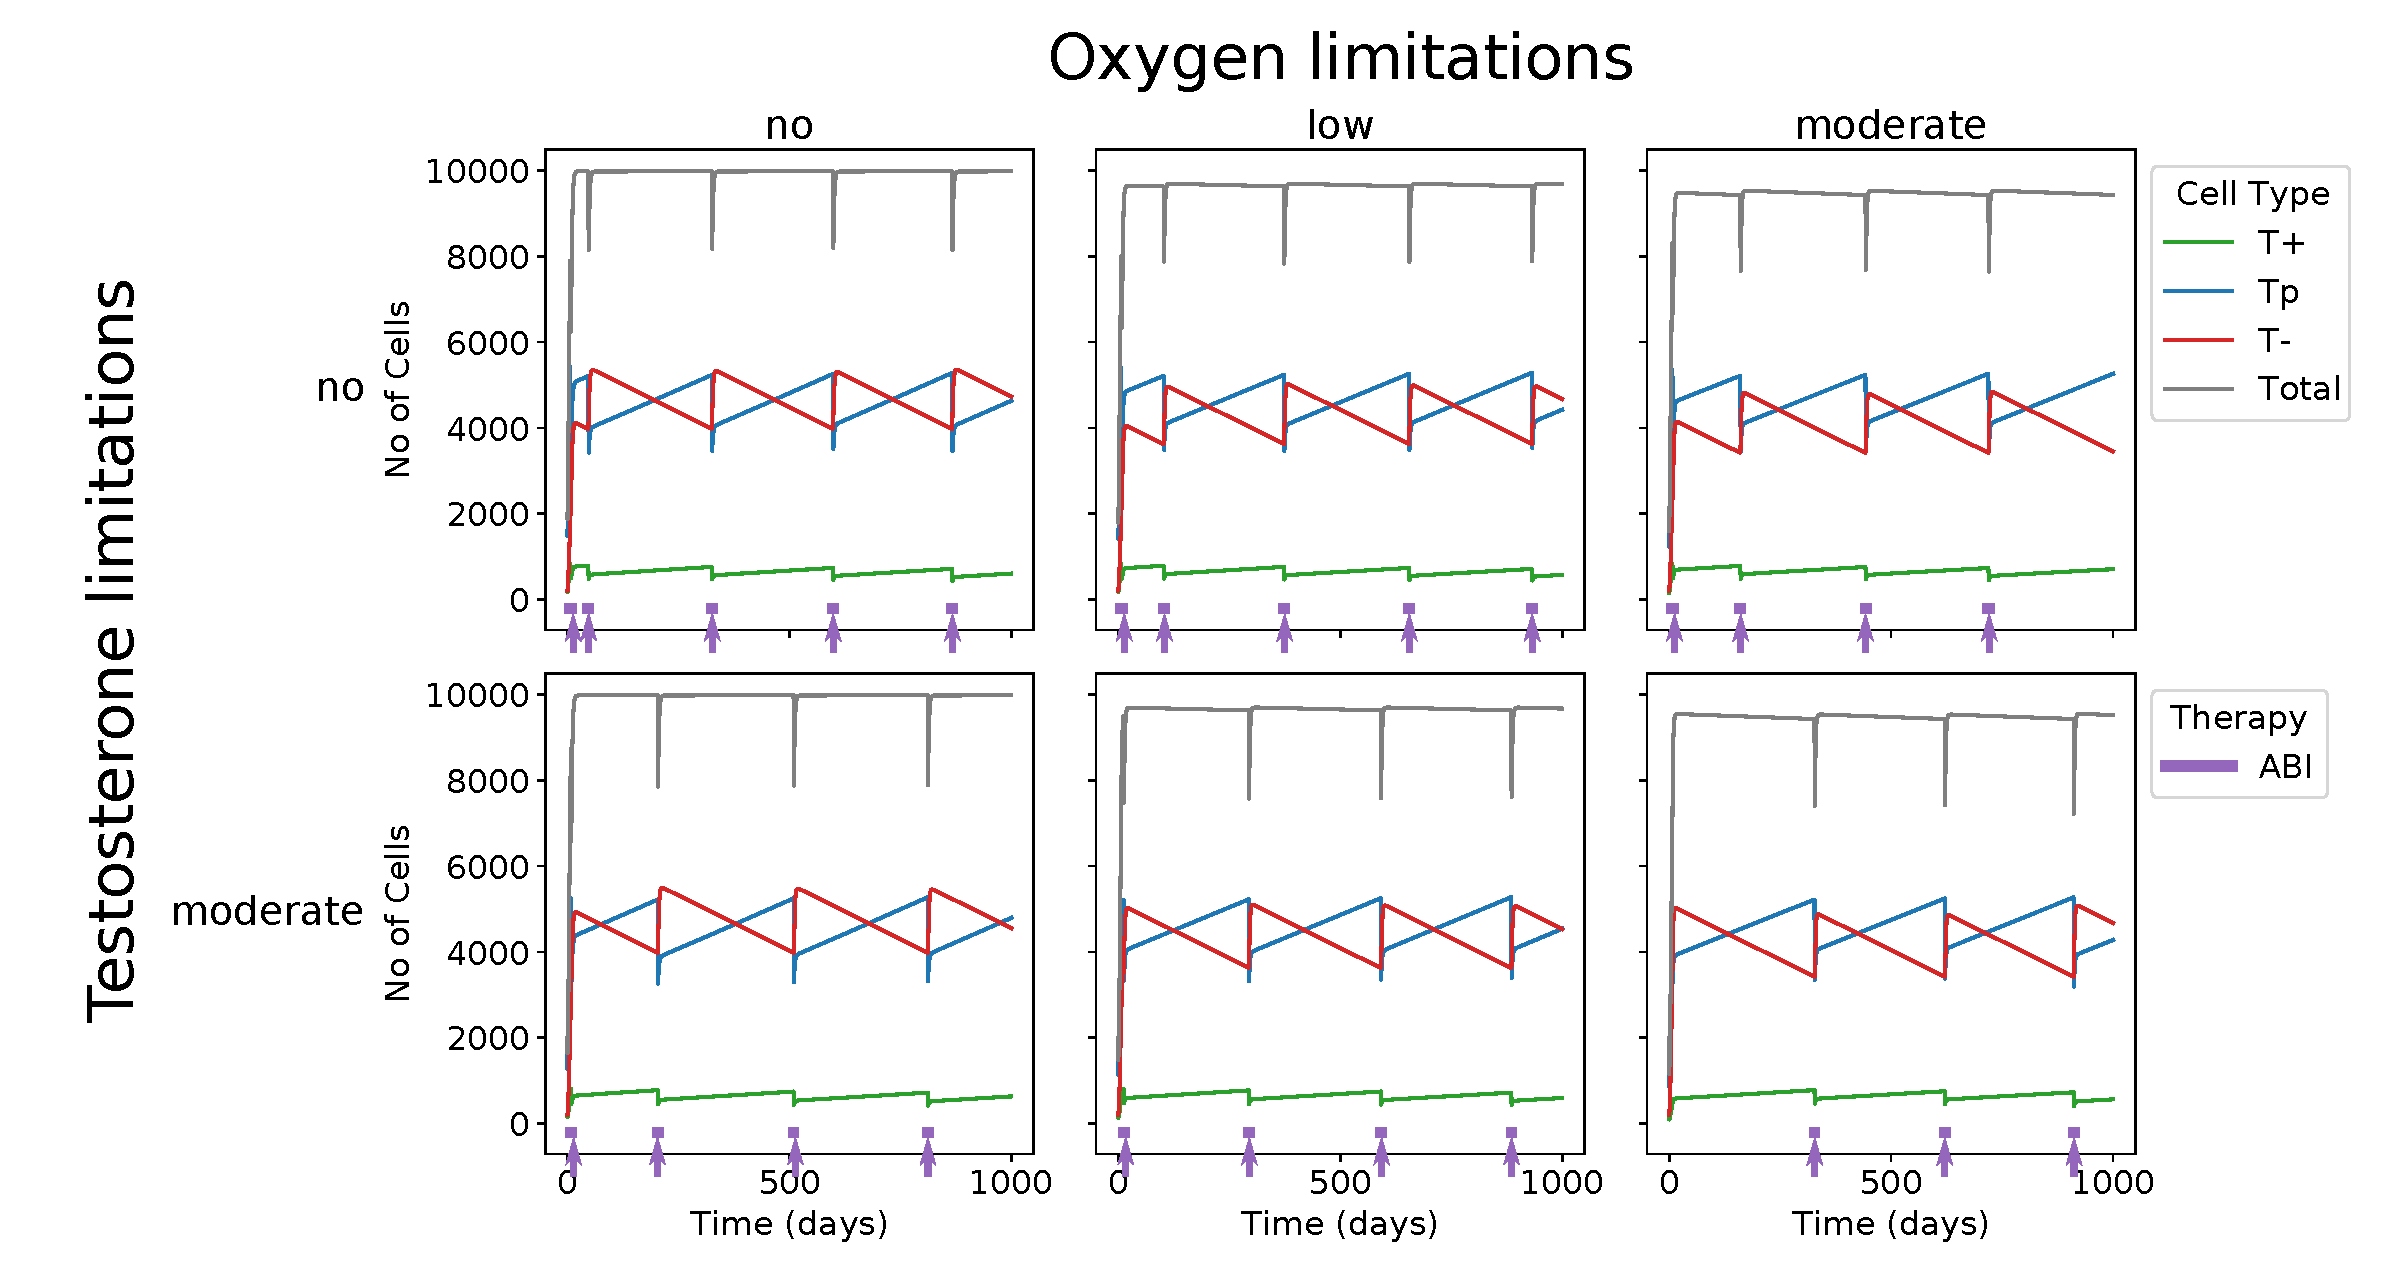
\includegraphics[width=\textwidth]{All3_therapy_8:1:1-2000}
      \caption{High $T^p$ seeding - 8:1:1}
    \end{subfigure}
    \caption{Time-series of all cell types with AT. C: $O_2$ limits, R: $test$ limits and SF: seeding propn. (On:6000, Off:4000)}
  \end{figure}
  \begin{columns}
    \begin{column}{0.5\textwidth}
      \begin{itemize}
        \item Higher $T^+ - T^p$: more treatable
        \item $test$ mod.: extinct from comp.
      \end{itemize}
    \end{column}
    \begin{column}{0.5\textwidth}
      \begin{itemize}
        \item Apply therapy - $T^-$ quickly replace \\
        $\rightarrow$ tot. popn. high
      \end{itemize}
    \end{column}
  \end{columns}
\end{frame}

\begin{frame}{AT w/ delay}
  \begin{figure}[h]
    \centering
    \begin{subfigure}[b]{0.48\textwidth}
      \centering
      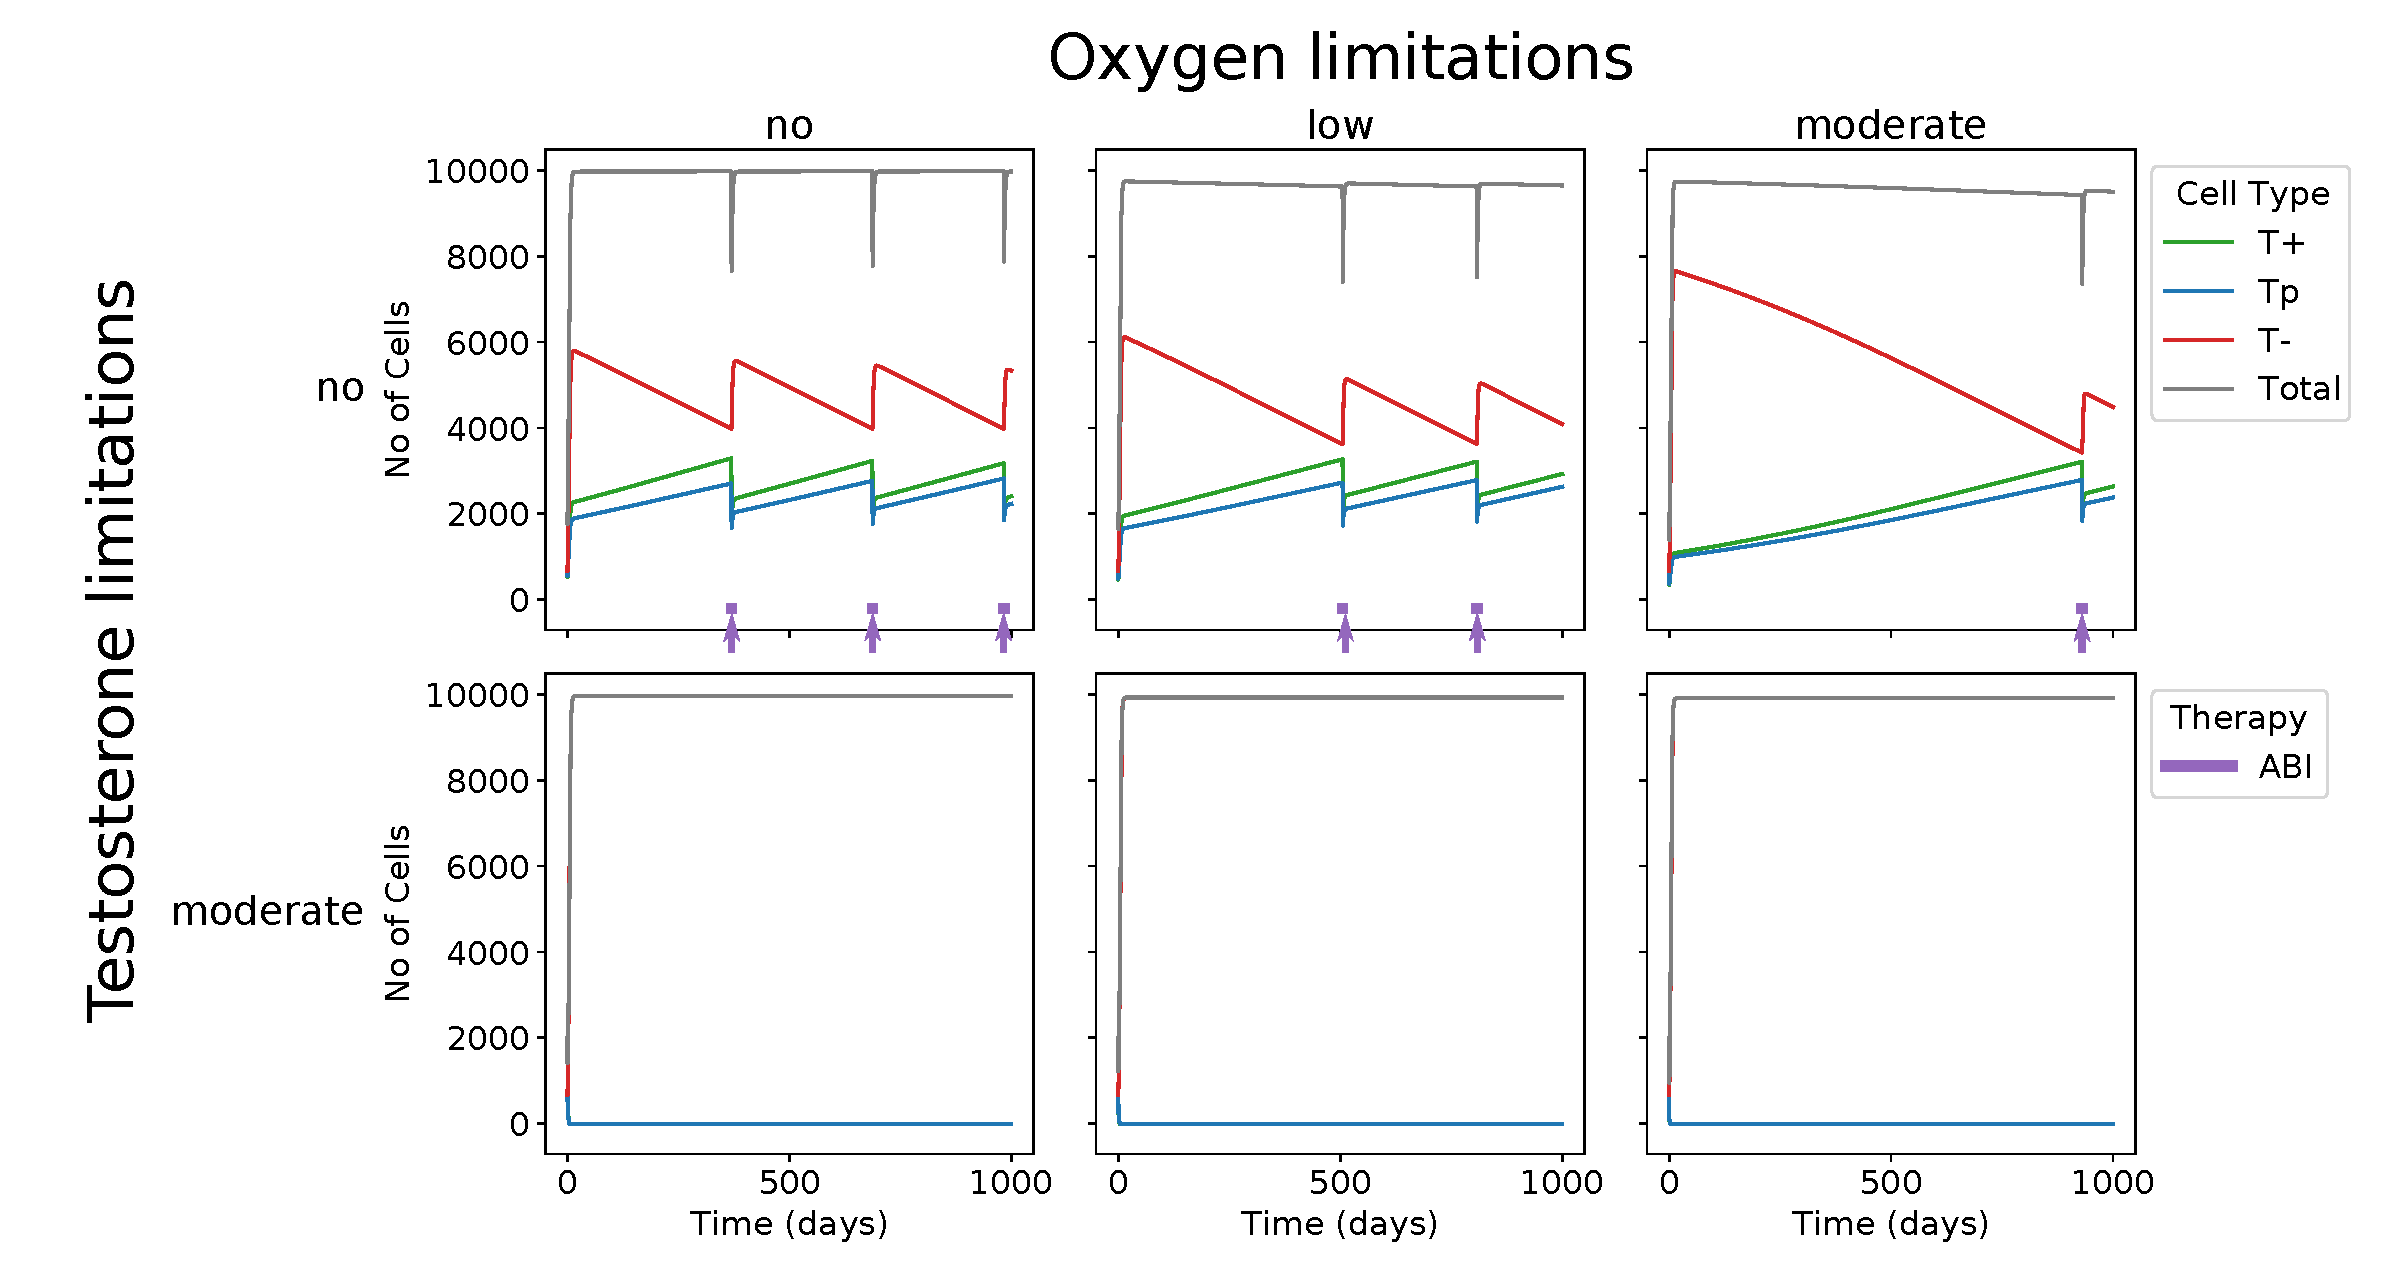
\includegraphics[width=\textwidth]{All3_therapy_200day_1:1:1}
      \caption{Equal seeding - 1:1:1}
    \end{subfigure}
    \begin{subfigure}[b]{0.48\textwidth}
      \centering
      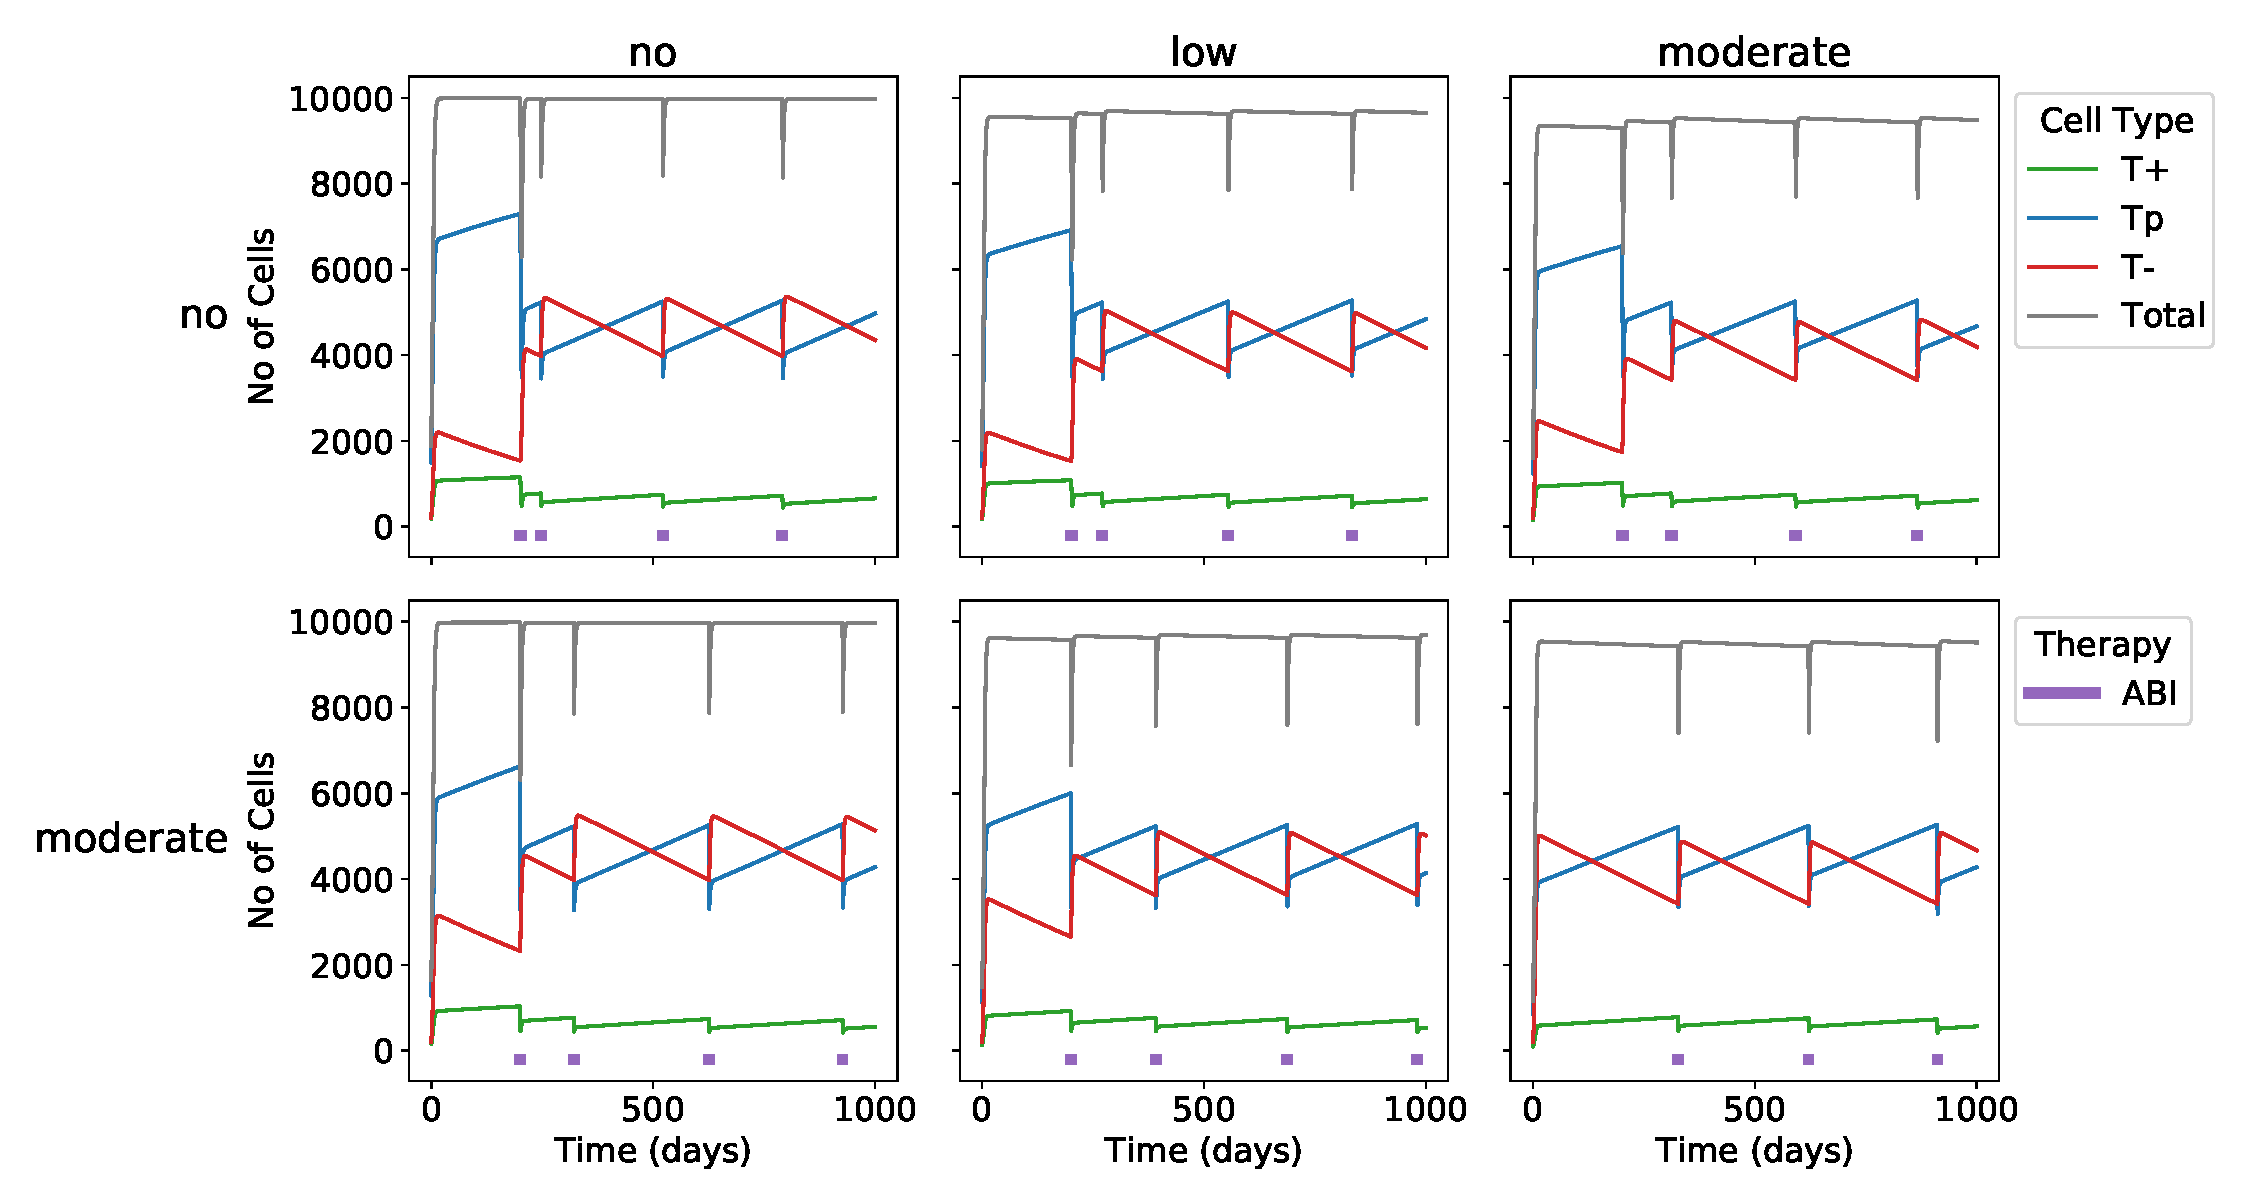
\includegraphics[width=\textwidth]{All3_therapy_200day_8:1:1}
      \caption{High $T^p$ seeding - 8:1:1}
    \end{subfigure}
    \caption{Time-series of all cell types with AT delayed by 200 days. C: $O_2$ limits, R: $test$ limits and SF: seeding propn. (On:6000, Off:4000)}
  \end{figure}
  \begin{columns}
    \begin{column}{0.5\textwidth}
      \begin{itemize}
        \item Speculate: delay $\rightarrow$ $T^+ - T^p$ $\uparrow$
      \end{itemize}
    \end{column}
    \begin{column}{0.5\textwidth}
      \begin{itemize}
        \item No advantage $\leftarrow$ no variability
        \item Physiological cost
      \end{itemize}
    \end{column}
  \end{columns}
\end{frame}

\begin{frame}{Combination AT}
  \begin{figure}[h]
    \centering
    \begin{subfigure}[b]{0.48\textwidth}
      \centering
      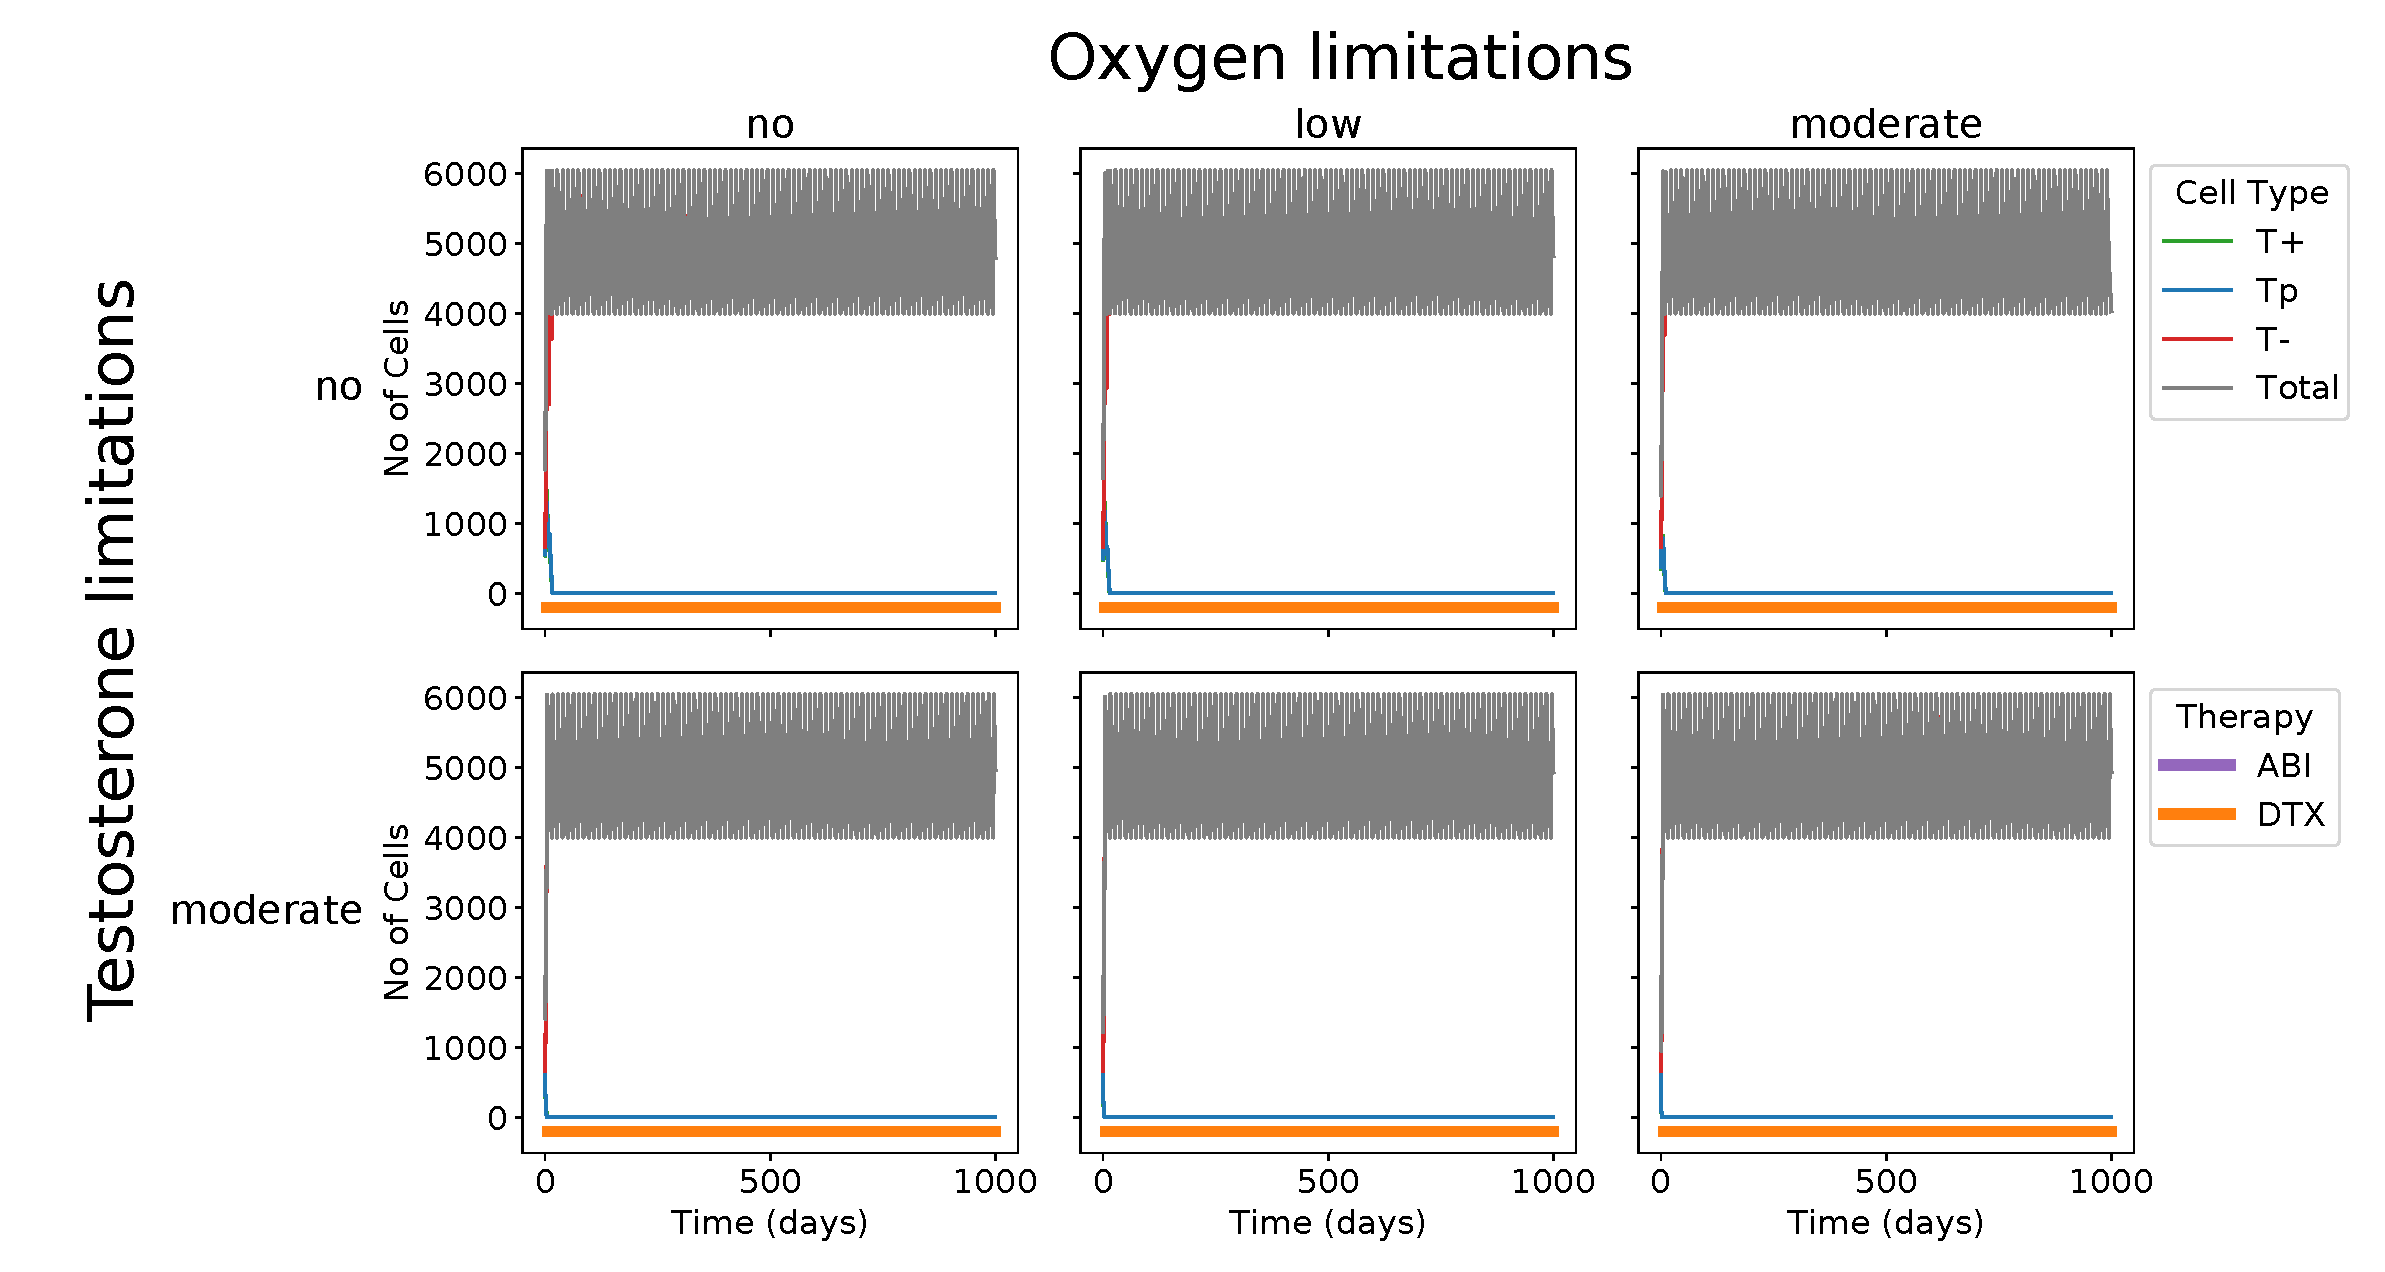
\includegraphics[width=\textwidth]{All3_therapy-combi_1:1:1}
      \caption{Equal seeding - 1:1:1}
    \end{subfigure}
    \begin{subfigure}[b]{0.48\textwidth}
      \centering
      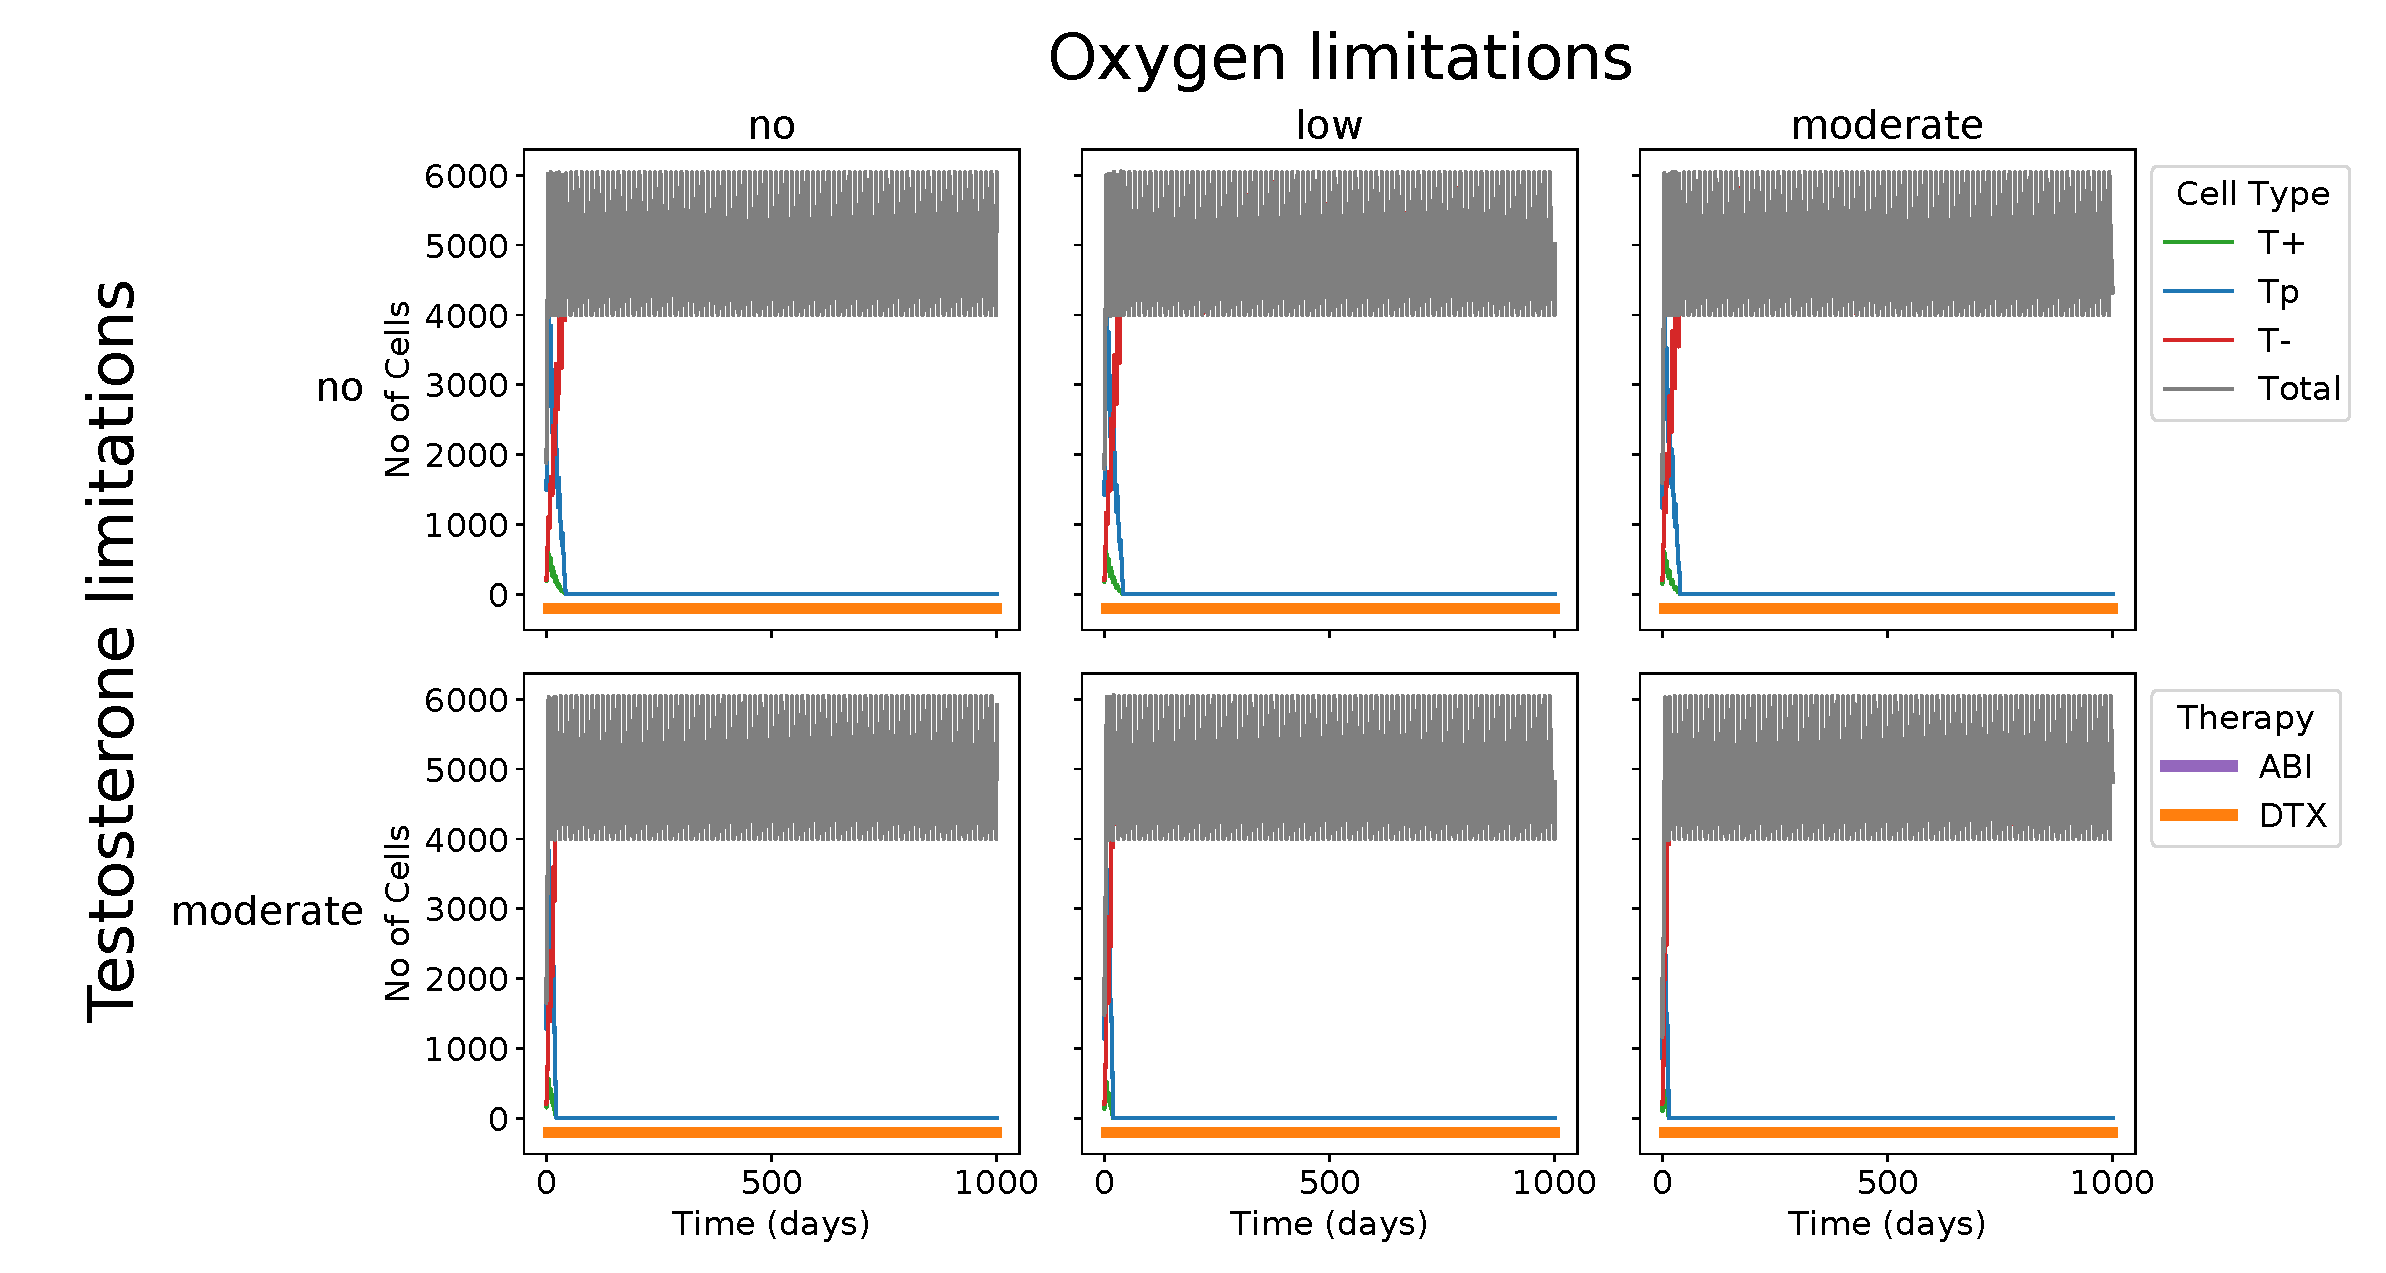
\includegraphics[width=\textwidth]{All3_therapy-combi_8:1:1}
      \caption{High $T^p$ seeding - 8:1:1}
    \end{subfigure}
    \caption{Time-series of all cell types with combination AT of abi and dtx. C: $O_2$ limits, R: $test$ limits and SF: seeding propn. abi(On:6000, Off:4000; $T^+ + T^p$), dtx(On:6000, Off:4000; $T^+ + T^p + T^-$)}
  \end{figure}
  \begin{columns}
    \begin{column}{0.5\textwidth}
      \begin{itemize}
        \item Hormone-specific + cytoxic \cite{West}
        \item Test-of-concept: abi - $T^+ - T^p$, dtx - total
      \end{itemize}
    \end{column}
    \begin{column}{0.5\textwidth}
      \begin{itemize}
        \item $-ve$ effect on $T^+ - T^p$ vs $+ve$ effect $\downarrow$ $T^-$
      \end{itemize}
    \end{column}
  \end{columns}
\end{frame}


\section{Conclusion}

\begin{frame}{Summary and Future directions}
  \begin{itemize}
    \item<1-> Resource levels can control strength of competition
    \item<2-> Balance of limitations promote coexistence
    \item<3-> With standard-of-care: testosterone limitation is increased leading to extinction
    \item<4-> With adaptive therapy: competitive release avoided
    \begin{itemize}
      \item Effectiveness depends on $T^+$ and $T^p$ population
      \item Population controlled by resource limitations
      \item Maximum limit on $T^+$ and $T^p$ by thresholds of adaptive therapy
    \end{itemize}
    \item<5-> Future directions:
    \begin{itemize}
      \item<6-> Make adaptive therapy effective at reducing tumour burden
      \item<7-> Dynamic thresholds for turning on/off based on composition of the tumour
      \item<8-> Different limitations for different cell types
    \end{itemize}
  \end{itemize}
\end{frame}

\begin{frame}{Acknowledgement}
  I would like to thank the following people:
  \begin{itemize}
    \item Supervisor: Prof. Sutirth Dey
    \item Expert: Dr. M.S. Madhusudhan
    \item Mentor: Vibishan B
    \item PBL Members
    \item Friends and Family
    \item KVPY and IISER Pune
  \end{itemize}
\end{frame}


\begin{frame}[allowframebreaks]
  \printbibliography
\end{frame}

\end{document}
